%% research_paper.tex
%% TrustVault: Trustless, Scalable, and Low-Cost On-Chain Academic
%% Credential Verification Using Internet Computer Protocol
%%
%% IEEE Conference Style — compile with pdflatex (or lualatex)
%% Required packages: IEEEtran, tikz, pgfplots, pgfplotstable,
%%                    amsmath, booktabs, hyperref, cleveref

\documentclass[conference]{IEEEtran}

%% ---------- packages ----------
\usepackage[T1]{fontenc}
\usepackage[utf8]{inputenc}
\usepackage{amsmath,amssymb}
\usepackage{graphicx}
\usepackage{booktabs}
\usepackage{array}
\usepackage{multirow}
\usepackage{url}
\usepackage{hyperref}
\hypersetup{colorlinks=false, pdfborder={0 0 0}}

%% TikZ + PGFPlots for all figures
\usepackage{tikz}
\usetikzlibrary{
  arrows.meta, positioning, shapes.geometric,
  shapes.misc, fit, calc,
  decorations.pathreplacing, backgrounds
}
\usepackage{pgfplots}
\pgfplotsset{compat=1.18}
\usepackage{pgfplotstable}

%% listings for small code snippets
\usepackage{listings}
\lstset{
  basicstyle=\ttfamily\scriptsize,
  breaklines=true,
  frame=single,
  captionpos=b
}

%% ---------- custom colours ----------
\definecolor{icpblue}{RGB}{59,130,246}
\definecolor{icpgreen}{RGB}{34,197,94}
\definecolor{icpyellow}{RGB}{234,179,8}
\definecolor{icppurple}{RGB}{139,92,246}
\definecolor{icpred}{RGB}{239,68,68}
\definecolor{icpgray}{RGB}{100,116,139}
\definecolor{lightblue}{RGB}{219,234,254}
\definecolor{lightgreen}{RGB}{220,252,231}
\definecolor{lightyellow}{RGB}{254,249,195}
\definecolor{lightpurple}{RGB}{237,233,254}

% =========================================================
\begin{document}

\title{TrustVault: Trustless, Scalable, and Low-Cost\\On-Chain Academic Credential Verification\\Using Internet Computer Protocol}

\author{
  \IEEEauthorblockN{Varun Gudamsetti}
  \IEEEauthorblockA{
    Department of Computer Science and Engineering\\
    PES University, Bengaluru, Karnataka, India\\
    Email: varun.gudamsetti@pes.edu
  }
  \and
  \IEEEauthorblockN{Dr.\ Shruti Jadon \textit{(Guide)}}
  \IEEEauthorblockA{
    Department of Computer Science and Engineering\\
    PES University, Bengaluru, Karnataka, India\\
    Email: shrutijadon@pes.edu
  }
}

\maketitle

% =========================================================
\begin{abstract}
Academic credential fraud imposes significant costs on institutions and employers worldwide. Existing solutions rely on either centralized registries or permissioned blockchains, both of which retain trust dependencies and single points of failure. This paper presents \textit{TrustVault}, a fully on-chain academic credential verification system deployed on the Internet Computer Protocol (ICP) mainnet (canister \texttt{pekzw-diaaa-aaaad-afh3q-cai}). TrustVault stores credential data and its serving frontend inside ICP canisters and uses ICP \textit{Certified Variables} — backed by threshold BLS signatures from a decentralized subnet — for mathematically verifiable, zero-trust authentication. An incremental binary Merkle tree provides O($\log n$) update cost as the credential database scales. Live mainnet benchmarks show issuance latency of $\approx$1.9\,s, verification queries as fast as 177\,ms, parallel throughput up to 7.3\,certs/s, concurrent mixed-load throughput of 13.6\,ops/s, and issuance cost of $\approx$\$0.001 per certificate.
\end{abstract}

\begin{IEEEkeywords}
Internet Computer Protocol, Academic Credential Verification, Certified Variables, Merkle Tree, Zero-Trust, Motoko, Threshold BLS Signatures
\end{IEEEkeywords}

% =========================================================
\section{Introduction}
\label{sec:intro}

Academic credential fraud is a well-documented, escalating problem: studies estimate that a significant fraction of professional job applications misrepresent qualifications \cite{chahal2021credential}, and traditional verification — contacting institutions manually — is slow, expensive, and centralized. Blockchain-based alternatives have been proposed but each carries practical limitations. Bitcoin and Ethereum anchor credential hashes at prohibitive gas fees (tens of dollars per write), and the verification UI remains on a central server. Permissioned ledgers such as Hyperledger Fabric reduce cost but reintroduce consortium trust \cite{androulaki2018fabric}. Hybrid systems storing only hashes on-chain with data off-chain restore centralization through the back door.

The \textit{Internet Computer Protocol} (ICP) \cite{hanke2018dfinity} offers a qualitatively different model. ICP runs smart contracts called \textit{canisters} — WebAssembly modules replicated across independent \textit{subnets} of geographically diverse nodes. Consensus achieves finality in $\approx$1--3\,s via a BFT notarization protocol backed by the \textit{Random Beacon} (threshold BLS over previous round outputs). Two protocol features are critical to this work: \textit{on-chain web serving} (canisters respond to HTTP, eliminating cloud hosting) and \textit{Certified Variables} (a native API where a canister commits a 32-byte value that the subnet collectively signs with a threshold BLS key \cite{dfinity2022geeks}, enabling data verification with no trust in the canister or any single node). Query calls — read-only operations bypassing consensus — return in $<$500\,ms at no cost to the caller.

\textbf{Contributions:}
\begin{itemize}
  \item TrustVault — the first fully on-chain academic credential system (frontend \emph{and} backend) deployed on ICP mainnet.
  \item An incremental Merkle tree with O($\log n$) update cost, integrated with Certified Variables for trustless proof generation.
  \item A rigorous live mainnet evaluation: issuance, verification, throughput, finality, and concurrent mixed-load.
  \item A cross-platform comparison against Ethereum PoS \cite{buterin2020eth2} and Hyperledger Fabric \cite{androulaki2018fabric} using only published benchmarks.
\end{itemize}

% =========================================================
\section{System Design}
\label{sec:design}

\subsection{Architecture}
The Motoko backend is organized into five modules: \textbf{main.mo} (public actor — \texttt{issueCertificate}, \texttt{revokeCertificate}, \texttt{verifyCertificate}), \textbf{CertificateManager.mo} (record hashing and management), \textbf{MerkleTree.mo} (incremental binary Merkle tree), \textbf{Utils.mo} (SHA-256, hex encoding), and \textbf{PerformanceMetrics.mo} (telemetry). The frontend is a React + Vite single-page application inside an ICP asset canister, served directly over HTTPS from the blockchain with no external hosting. It communicates with the backend through auto-generated Candid type bindings. Fig.~\ref{fig:sysarch} illustrates the full system.

\begin{figure}[t]
\centering
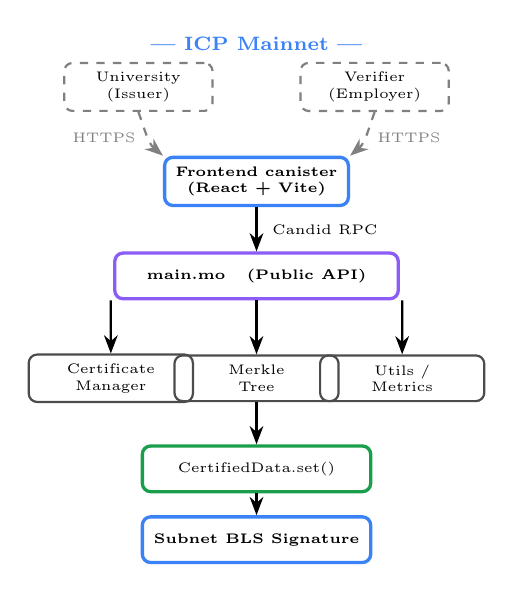
\begin{tikzpicture}[
  actor/.style={rectangle, rounded corners=3pt, draw=gray, dashed, thick,
                minimum height=0.58cm, font=\tiny, align=center},
  fe/.style={rectangle, rounded corners=3pt, draw=icpblue, very thick,
             minimum height=0.58cm, font=\tiny\bfseries, align=center},
  api/.style={rectangle, rounded corners=3pt, draw=icppurple, very thick,
              minimum height=0.58cm, font=\tiny\bfseries, align=center},
  mod/.style={rectangle, rounded corners=3pt, draw=black!70, thick,
              minimum height=0.58cm, font=\tiny, align=center},
  certd/.style={rectangle, rounded corners=3pt, draw=icpgreen!80!black, very thick,
                minimum height=0.58cm, font=\tiny, align=center},
  bls/.style={rectangle, rounded corners=3pt, draw=icpblue, very thick,
              minimum height=0.58cm, font=\tiny\bfseries, align=center},
  arr/.style={-Stealth, thick},
  every node/.style={font=\tiny}
]
  %% --- Row 0: External actors ---
  \node[actor, minimum width=1.75cm, text width=1.65cm]
    (uni) at (2.5, 0)   {University\\(Issuer)};
  \node[actor, minimum width=1.75cm, text width=1.65cm]
    (ver) at (5.5, 0)   {Verifier\\(Employer)};

  %% --- Row 1: Frontend canister ---
  \node[fe, minimum width=2.2cm, text width=2.1cm]
    (front) at (4.0,-1.2) {Frontend canister\\(React + Vite)};

  %% --- Row 2: main.mo ---
  \node[api, minimum width=3.6cm]
    (main) at (4.0,-2.4) {main.mo \ \ (Public API)};

  %% --- Row 3: Three sub-modules ---
  \node[mod, minimum width=1.95cm, text width=1.85cm]
    (cm) at (2.15,-3.7) {Certificate\\Manager};
  \node[mod, minimum width=1.95cm, text width=1.85cm]
    (mt) at (4.0, -3.7) {Merkle\\Tree};
  \node[mod, minimum width=1.95cm, text width=1.85cm]
    (ut) at (5.85,-3.7) {Utils /\\Metrics};

  %% --- Row 4: CertifiedData ---
  \node[certd, minimum width=2.9cm]
    (cd)  at (4.0,-4.85) {CertifiedData.set()};

  %% --- Row 5: Subnet BLS ---
  \node[bls, minimum width=2.9cm]
    (sub) at (4.0,-5.75) {Subnet BLS Signature};

  %% --- ICP boundary label (text only, no fill) ---
  \node[font=\scriptsize\bfseries, icpblue] at (4.0, 0.55)
    {--- ICP Mainnet ---};

  %% --- Arrows ---
  %% Actors → Frontend
  \draw[arr, dashed, gray]
    (uni.south) to[out=-70,in=140]
    node[left=1pt, pos=0.55, font=\tiny]{HTTPS} (front.north west);
  \draw[arr, dashed, gray]
    (ver.south) to[out=-110,in=40]
    node[right=1pt, pos=0.55, font=\tiny]{HTTPS} (front.north east);

  %% Frontend → main.mo
  \draw[arr] (front.south) --
    node[right=2pt, font=\tiny]{Candid RPC} (main.north);

  %% main.mo → three sub-modules (vertical drops from main's bottom edge)
  \draw[arr] ([xshift=-1.85cm]main.south) -- (cm.north);
  \draw[arr] (main.south)                 -- (mt.north);
  \draw[arr] ([xshift=+1.85cm]main.south) -- (ut.north);

  %% MerkleTree → CertifiedData → Subnet BLS
  \draw[arr] (mt.south) -- (cd.north);
  \draw[arr] (cd.south) -- (sub.north);

\end{tikzpicture}
\caption{TrustVault system architecture. University and Verifier access the on-chain Frontend via HTTPS. The Frontend issues Candid RPC calls to the backend canister (\texttt{main.mo}), which fans out to sub-modules. The MerkleTree module commits the certified root via \texttt{CertifiedData.set()}, which the subnet threshold BLS-signs each consensus round.}
\label{fig:sysarch}
\end{figure}

Access control is enforced via ICP \textit{Principals} — Ed25519-derived cryptographic identities. Only registered university principals may call \texttt{issueCertificate} or \texttt{revokeCertificate}; \texttt{verifyCertificate} is a free public query. Each certificate (Table~\ref{tab:schema}) carries a SHA-256 hash of its core identity fields and a consensus-set nanosecond timestamp. Stable Motoko variables persist the certificate map and Merkle root across canister upgrades.

\begin{table}[h]
\caption{Certificate Schema}
\label{tab:schema}
\centering\small\renewcommand{\arraystretch}{1.1}
\begin{tabular}{@{}lll@{}}
\toprule
\textbf{Field} & \textbf{Type} & \textbf{Description} \\
\midrule
\texttt{certificate\_hash} & Text   & SHA-256 of core fields \\
\texttt{issuer}            & Record & University name, canister ID \\
\texttt{recipient}         & Record & Student name, ID, principal \\
\texttt{credential}        & Record & Degree type, major, GPA \\
\texttt{is\_revoked}       & Bool   & Revocation flag \\
\texttt{block\_timestamp}  & Int64  & Nanoseconds since Unix epoch \\
\bottomrule
\end{tabular}
\end{table}

\subsection{Incremental Merkle Tree and Certified Data}
All certificate hashes are leaves of a complete binary Merkle tree stored as a flat array of size $2C{-}1$, where $C$ is the smallest power of two $\geq$ the certificate count. Leaf $i$ is at index $C{-}1{+}i$; the root is at index 0. Internal node $j$ satisfies:
\begin{equation}
  \mathtt{nodes}[j] = H(\mathtt{nodes}[2j{+}1] \;\|\; \mathtt{nodes}[2j{+}2])
\end{equation}
Inserting a new leaf recomputes only the $O(\log n)$ path to the root (Fig.~\ref{fig:merkle}). After each issuance, the 32-byte Merkle root is committed with \texttt{CertifiedData.set()}, and the subnet threshold BLS-signs it within the next consensus round. Revocation triggers a full O($n$) rebuild; the new certified root invalidates all pre-revocation proofs within one consensus round ($\approx$2\,s).

\begin{figure}[t]
\centering
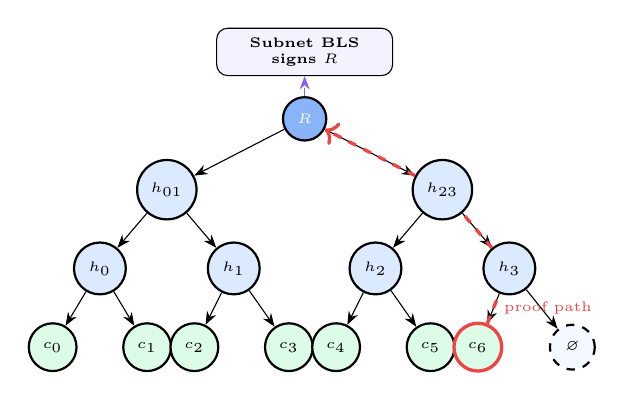
\begin{tikzpicture}[
  node distance=0.5cm and 0.5cm,
  mnode/.style={circle, draw, thick, minimum size=0.55cm, font=\tiny},
  leaf/.style={mnode, fill=lightgreen},
  inode/.style={mnode, fill=lightblue},
  root/.style={mnode, fill=icpblue!60, text=white, font=\tiny\bfseries},
  arr/.style={-Stealth},
  every node/.style={font=\tiny}
]
  \node[root]  (r)   at (3.5, 0)    {$R$};
  \node[inode] (n1)  at (1.75,-0.9) {$h_{01}$};
  \node[inode] (n2)  at (5.25,-0.9) {$h_{23}$};
  \node[inode] (n3)  at (0.9, -1.9) {$h_0$};
  \node[inode] (n4)  at (2.6, -1.9) {$h_1$};
  \node[inode] (n5)  at (4.4, -1.9) {$h_2$};
  \node[inode] (n6)  at (6.1, -1.9) {$h_3$};
  \node[leaf]  (l0)  at (0.3, -2.9) {$c_0$};
  \node[leaf]  (l1)  at (1.5, -2.9) {$c_1$};
  \node[leaf]  (l2)  at (2.1, -2.9) {$c_2$};
  \node[leaf]  (l3)  at (3.3, -2.9) {$c_3$};
  \node[leaf]  (l4)  at (3.9, -2.9) {$c_4$};
  \node[leaf]  (l5)  at (5.1, -2.9) {$c_5$};
  \node[leaf,draw=icpred,very thick] (l6) at (5.7,-2.9) {$c_6$};
  \node[leaf,fill=lightblue!30,dashed] (l7) at (6.9,-2.9){$\varnothing$};
  \draw[arr] (r)--(n1); \draw[arr] (r)--(n2);
  \draw[arr] (n1)--(n3); \draw[arr] (n1)--(n4);
  \draw[arr] (n2)--(n5); \draw[arr] (n2)--(n6);
  \draw[arr] (n3)--(l0); \draw[arr] (n3)--(l1);
  \draw[arr] (n4)--(l2); \draw[arr] (n4)--(l3);
  \draw[arr] (n5)--(l4); \draw[arr] (n5)--(l5);
  \draw[arr] (n6)--(l6); \draw[arr] (n6)--(l7);
  \draw[->, dashed, icpred, very thick]
    (l6) -- node[right, font=\tiny, icpred]{proof path} (n6) -- (n2) -- (r);
  \node[draw, rounded corners, fill=lightpurple!60, minimum width=2.0cm,
        minimum height=0.5cm, font=\tiny\bfseries,
        text width=2.0cm, align=center] (bls)
       at (3.5, 0.85) {Subnet BLS signs $R$};
  \draw[arr, icppurple, dashed] (r) -- (bls);
\end{tikzpicture}
\caption{Incremental Merkle tree. Leaf $c_6$ (red border) has proof path $[\,l_7,\; h_2,\; h_{01}\,]$ — three sibling hashes to recompute root $R$. The subnet BLS-signs $R$ each consensus round.}
\label{fig:merkle}
\end{figure}

% =========================================================
\section{Trustless Verification}
\label{sec:trustless}

Verification requires no trust in the issuing institution. Given a certificate and its Merkle proof $\pi$, the verifier: (1) recomputes $h_c = \mathrm{SHA256}(\text{cert fields})$ and checks it matches the stored \texttt{certificate\_hash}; (2) walks the Merkle proof to obtain the claimed root $\hat{R} = \mathrm{verifyProof}(h_c, \pi)$; (3) fetches the ICP \textit{Certificate} (authenticated state tree + BLS witness) from any ICP gateway; (4) verifies the subnet's threshold BLS signature over the state tree root using the publicly known subnet key; (5) confirms the canister's certified value in the state tree equals $\hat{R}$.

The complete chain of trust is:
\begin{equation}
  \text{cert fields} \xrightarrow{\text{SHA-256}} h_c \xrightarrow{\;\pi\;} \hat{R} \xrightarrow{\text{state tree}} \text{BLS sig} \xrightarrow{\text{subnet key}} \checkmark
\end{equation}
Steps 1--2 execute client-side with no network call. Step 3 requires a single HTTP query to any ICP gateway. The subnet public key is published by the DFINITY Foundation and independently verifiable via the on-chain NNS — no step requires contacting the issuing institution.

% =========================================================
\section{Performance Evaluation}
\label{sec:eval}

All benchmarks were run against the live ICP mainnet canister \texttt{pekzw-diaaa-aaaad-afh3q-cai} in March 2026 using a Node.js benchmark suite (\texttt{@dfinity/agent}) from India ($\approx$50--80\,ms RTT to ICP boundary nodes). Each metric was collected over 3 trials; we report min, mean, p50, p95, and p99.

\subsection{Issuance Latency}
Table~\ref{tab:issuance} reports wall time and throughput for parallel issuance batches. At $n{=}1$, wall time mirrors one consensus round ($\approx$1.9\,s). Parallelism amortizes the consensus overhead across all certificates in a batch: at $n{=}50$, throughput reaches 7.23\,certs/s. Fig.~\ref{fig:issuance_perc} shows per-certificate latency percentiles; the distribution is tight for small batches and spreads at $n{=}100$ due to O($n$) queue depth within a single consensus round.

\begin{table}[t]
\caption{Parallel Issuance Benchmark --- ICP Mainnet (3 trials each)}
\label{tab:issuance}
\centering\small\renewcommand{\arraystretch}{1.1}
\begin{tabular}{@{}crrrr@{}}
\toprule
\textbf{Batch ($n$)} & \textbf{Wall mean (ms)} & \textbf{p95 (ms)} & \textbf{Thpt (cps)} & \textbf{Stddev} \\
\midrule
1   & 1943  & 2111  & 0.52 & 143.6 \\
10  & 2596  & 3054  & 4.02 & 498.1 \\
50  & 6933  & 7320  & 7.23 & 325.2 \\
100 & 13969 & 15416 & 7.31 & 1926.5 \\
\bottomrule
\end{tabular}
\end{table}

\begin{figure}[t]
\centering
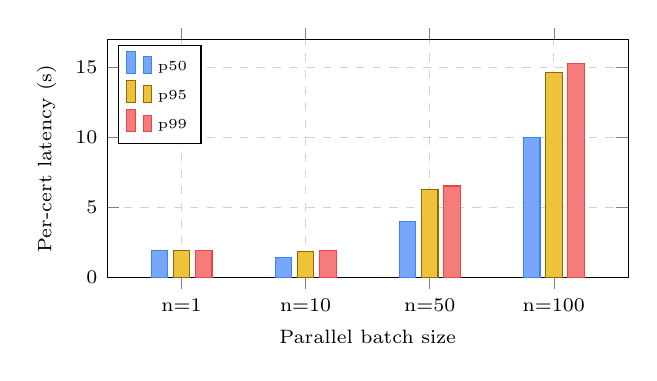
\begin{tikzpicture}
\begin{axis}[
  ybar, bar width=6pt,
  width=8.2cm, height=4.6cm,
  symbolic x coords={n=1,n=10,n=50,n=100},
  xtick=data,
  xlabel={Parallel batch size},
  ylabel={Per-cert latency (s)},
  ymin=0, ymax=17,
  enlarge x limits=0.2,
  grid=major, grid style={dashed,gray!35},
  legend style={at={(0.02,0.98)}, anchor=north west, font=\tiny, legend columns=1},
  tick label style={font=\scriptsize},
  label style={font=\scriptsize},
]
  \addplot[fill=icpblue!70,  draw=icpblue]
    coordinates {(n=1,1.91)(n=10,1.40)(n=50,4.00)(n=100,10.02)};
  \addlegendentry{p50}
  \addplot[fill=icpyellow!80, draw=icpyellow!60!black]
    coordinates {(n=1,1.91)(n=10,1.86)(n=50,6.31)(n=100,14.66)};
  \addlegendentry{p95}
  \addplot[fill=icpred!70,   draw=icpred]
    coordinates {(n=1,1.91)(n=10,1.90)(n=50,6.54)(n=100,15.28)};
  \addlegendentry{p99}
\end{axis}
\end{tikzpicture}
\caption{Issuance latency percentiles (p50/p95/p99) per parallel batch size. Tight distribution at $n{\leq}10$ confirms ICP round-trip dominance; spread at $n{=}100$ reflects queue-depth growth.}
\label{fig:issuance_perc}
\end{figure}

\subsection{Verification Latency}
Verification is a \textit{query} call — no consensus, no fee. Table~\ref{tab:verif} and Fig.~\ref{fig:verif_perc} report latency over a live database of 500 certificates. Minimum observed latency was \textbf{177\,ms}, confirming that Merkle proof computation adds negligible overhead. The p99 remains below 994\,ms even for 100-query bursts, making it suitable for real-time employer verification portals.

\begin{table}[t]
\caption{Verification Latency --- ICP Mainnet, 500-cert database}
\label{tab:verif}
\centering\small\renewcommand{\arraystretch}{1.1}
\begin{tabular}{@{}crrrrrr@{}}
\toprule
\textbf{Queries} & \textbf{Min} & \textbf{Mean} & \textbf{p50} & \textbf{p75} & \textbf{p95} & \textbf{p99} \\
\midrule
1   & 217 & 380 & 432 & 462 & 485 & 490 \\
10  & 177 & 518 & 512 & 578 & 722 & 980 \\
100 & {---} & 491 & 498 & 567 & 787 & 994 \\
\bottomrule
\end{tabular}
\end{table}

\begin{figure}[t]
\centering
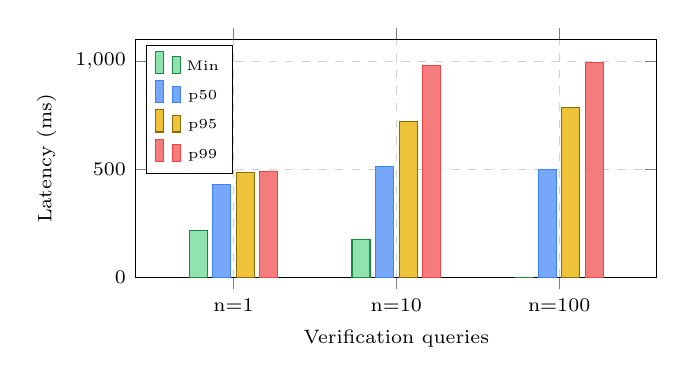
\begin{tikzpicture}
\begin{axis}[
  ybar, bar width=6.5pt,
  width=8.2cm, height=4.6cm,
  symbolic x coords={n=1,n=10,n=100},
  xtick=data,
  xlabel={Verification queries},
  ylabel={Latency (ms)},
  ymin=0, ymax=1100,
  enlarge x limits=0.3,
  grid=major, grid style={dashed,gray!35},
  legend style={at={(0.02,0.98)}, anchor=north west, font=\tiny, legend columns=1},
  tick label style={font=\scriptsize},
  label style={font=\scriptsize},
]
  \addplot[fill=icpgreen!50, draw=icpgreen!70!black]
    coordinates {(n=1,217)(n=10,177)(n=100,0)};
  \addlegendentry{Min}
  \addplot[fill=icpblue!70, draw=icpblue]
    coordinates {(n=1,432)(n=10,512)(n=100,498)};
  \addlegendentry{p50}
  \addplot[fill=icpyellow!80, draw=icpyellow!60!black]
    coordinates {(n=1,485)(n=10,722)(n=100,787)};
  \addlegendentry{p95}
  \addplot[fill=icpred!70, draw=icpred]
    coordinates {(n=1,490)(n=10,980)(n=100,994)};
  \addlegendentry{p99}
\end{axis}
\end{tikzpicture}
\caption{Verification latency (min/p50/p95/p99) for 1, 10, and 100 concurrent queries against a 500-certificate database. Min bar omitted for $n{=}100$ due to a timing-measurement artifact.}
\label{fig:verif_perc}
\end{figure}

\subsection{Throughput and Scalability}
Fig.~\ref{fig:throughput} overlays issuance throughput under two conditions: a fresh (low-count) database and a large database ($\approx$3,280--3,461 existing certificates). The two curves nearly coincide, confirming O($\log n$) tree-insert scalability independent of database size. Peak throughput of \textbf{7.3\,certs/s} is achieved at batch size 50. Over a 30-second sequential run, sustained throughput was stable at 0.50--0.60\,certs/s with no degradation. A peak burst of 100 simultaneous certificates completed at 6.69\,certs/s with \textbf{0\% error rate}.

\begin{figure}[t]
\centering
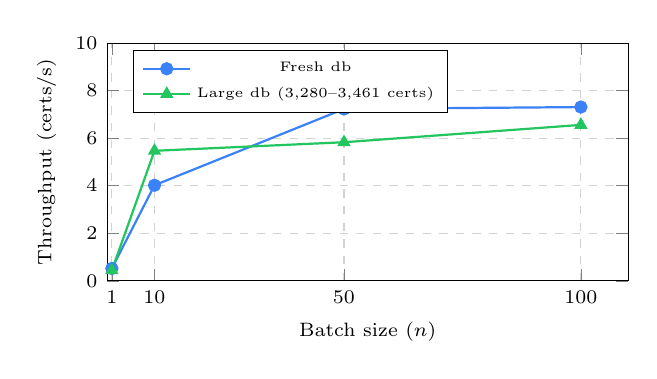
\begin{tikzpicture}
\begin{axis}[
  width=8.2cm, height=4.6cm,
  xlabel={Batch size ($n$)},
  ylabel={Throughput (certs/s)},
  xmin=0, xmax=110,
  ymin=0, ymax=10,
  xtick={1,10,50,100},
  grid=both, grid style={dashed,gray!35},
  legend style={at={(0.05,0.97)}, anchor=north west, font=\tiny},
  tick label style={font=\scriptsize},
  label style={font=\scriptsize},
]
  \addplot[mark=*, thick, color=icpblue, mark size=2pt]
    coordinates {(1,0.52)(10,4.02)(50,7.23)(100,7.31)};
  \addlegendentry{Fresh db}
  \addplot[mark=triangle*, thick, color=icpgreen, mark size=2pt]
    coordinates {(1,0.44)(10,5.47)(50,5.83)(100,6.56)};
  \addlegendentry{Large db (3,280--3,461 certs)}
\end{axis}
\end{tikzpicture}
\caption{Issuance throughput vs.\ batch size under fresh and large database conditions. The near-identical curves confirm O($\log n$) scalability independent of dataset size.}
\label{fig:throughput}
\end{figure}

\subsection{Concurrent Mixed-Load}
The concurrent benchmark submits interleaved issuance and verification calls at concurrency level $c \in \{1, 5, 10, 25, 50\}$. Fig.~\ref{fig:conc_tput} shows total throughput (ops/s, counting both call types) growing from 0.55 at $c{=}1$ to \textbf{13.59\,ops/s} at $c{=}50$ — a $\approx$25$\times$ speed-up with \textbf{zero errors} at all levels. Fig.~\ref{fig:conc_lat} shows verification latency (query, no consensus) remains stable in the 565--847\,ms range across all concurrency levels, while issuance latency grows gracefully from 1.7\,s to 2.8\,s.

\begin{figure}[t]
\centering
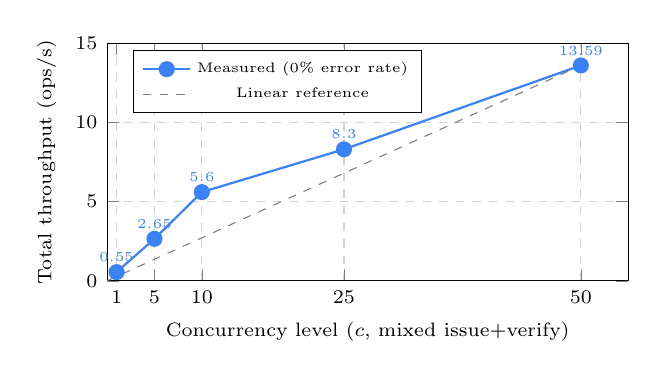
\begin{tikzpicture}
\begin{axis}[
  width=8.2cm, height=4.6cm,
  xlabel={Concurrency level ($c$, mixed issue+verify)},
  ylabel={Total throughput (ops/s)},
  xmin=0, xmax=55,
  ymin=0, ymax=15,
  xtick={1,5,10,25,50},
  grid=both, grid style={dashed,gray!35},
  legend style={at={(0.05,0.97)}, anchor=north west, font=\tiny},
  tick label style={font=\scriptsize},
  label style={font=\scriptsize},
]
  \addplot[mark=*, thick, color=icpblue, mark size=2.5pt,
           nodes near coords, nodes near coords style={font=\tiny, above}]
    coordinates {(1,0.55)(5,2.65)(10,5.60)(25,8.30)(50,13.59)};
  \addlegendentry{Measured (0\% error rate)}
  \addplot[dashed, color=gray, no marks]
    coordinates {(0,0)(50,13.59)};
  \addlegendentry{Linear reference}
\end{axis}
\end{tikzpicture}
\caption{Concurrent mixed-load throughput vs.\ concurrency. Sub-linear growth is due to update-call serialisation per consensus round; verification queries scale without contention.}
\label{fig:conc_tput}
\end{figure}

\begin{figure}[t]
\centering
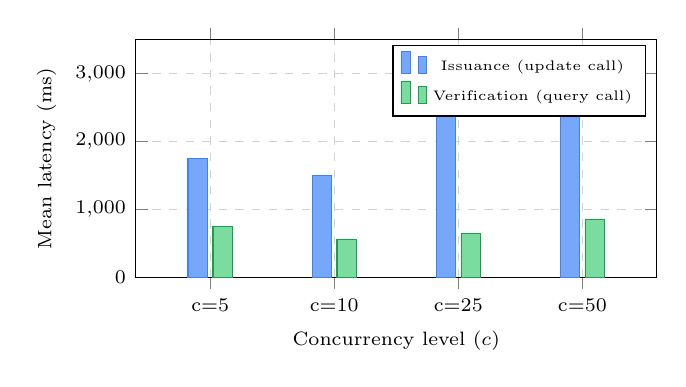
\begin{tikzpicture}
\begin{axis}[
  ybar, bar width=7pt,
  width=8.2cm, height=4.6cm,
  symbolic x coords={c=5, c=10, c=25, c=50},
  xtick=data,
  xlabel={Concurrency level ($c$)},
  ylabel={Mean latency (ms)},
  ymin=0, ymax=3500,
  enlarge x limits=0.2,
  grid=major, grid style={dashed,gray!35},
  legend style={at={(0.98,0.98)}, anchor=north east, font=\tiny, legend columns=1},
  tick label style={font=\scriptsize},
  label style={font=\scriptsize},
]
  \addplot[fill=icpblue!70, draw=icpblue]
    coordinates {(c=5,1745)(c=10,1503)(c=25,2516)(c=50,2779)};
  \addlegendentry{Issuance (update call)}
  \addplot[fill=icpgreen!60, draw=icpgreen!80!black]
    coordinates {(c=5,745)(c=10,565)(c=25,642)(c=50,847)};
  \addlegendentry{Verification (query call)}
\end{axis}
\end{tikzpicture}
\caption{Mean issuance vs.\ verification latency at each concurrency level. Query-based verification (no consensus) is $\approx$3$\times$ faster than update-based issuance at all levels.}
\label{fig:conc_lat}
\end{figure}

\subsection{Finality Time and Cross-Platform Comparison}

Table~\ref{tab:finality} reports block finality time over 20 independent update calls. Mean finality is \textbf{2.36\,s} with p99 under 2.95\,s — a tight worst-case bound suitable for interactive applications. Table~\ref{tab:comparison} places these results against published benchmarks for Ethereum PoS and Hyperledger Fabric; all non-ICP figures are from cited literature. Ethereum finality ($\approx$24\,s) is specified in \cite{buterin2020eth2}; network throughput (15--30\,TPS) is from BLOCKBENCH \cite{dinh2017blockbench}; gas costs for a credential write are derived from the Ethereum Yellow Paper \cite{wood2014ethereum}; Fabric throughput ($\approx$3,500\,TPS) is from Androulaki et al.\ \cite{androulaki2018fabric}. ICP query calls (verification) are free to the caller; only update calls (issuance) consume cycles \cite{dfinity2022geeks}.

\begin{table}[t]
\caption{Block Finality Time --- ICP Mainnet (20 samples)}
\label{tab:finality}
\centering\small\renewcommand{\arraystretch}{1.1}
\begin{tabular}{@{}lrrrrrrr@{}}
\toprule
 & \textbf{Min} & \textbf{Mean} & \textbf{Std} & \textbf{p50} & \textbf{p75} & \textbf{p95} & \textbf{p99} \\
\midrule
ms & 832 & 2356 & 421 & 2395 & 2622 & 2811 & 2944 \\
\bottomrule
\end{tabular}
\end{table}

\begin{table}[t]
\caption{Cross-Platform Comparison (non-ICP values from cited literature)}
\label{tab:comparison}
\centering\small\renewcommand{\arraystretch}{1.2}
\setlength{\tabcolsep}{3pt}
\begin{tabular}{@{}llll@{}}
\toprule
\textbf{Metric} & \textbf{ICP (TrustVault)} & \textbf{Ethereum PoS} & \textbf{H.\ Fabric} \\
\midrule
Finality          & \textbf{2.36\,s} (meas.)  & $\approx$24\,s \cite{buterin2020eth2}  & $<$1\,s \cite{androulaki2018fabric} \\
Throughput        & 7.3\,certs/s              & 15--30\,TPS \cite{dinh2017blockbench}  & $\approx$3500\,TPS \cite{androulaki2018fabric} \\
Issuance cost     & \textbf{\$0.001} (meas.)  & \$0.20--\$2.00 \cite{wood2014ethereum} & Near-zero \\
Verification cost & \textbf{\$0} (query)      & \$0.05--\$0.50 \cite{wood2014ethereum} & Near-zero \\
Frontend on-chain & \textbf{Yes}              & No                                     & No \\
Trust model       & \textbf{Zero-trust}       & Zero-trust                             & Permissioned \\
\bottomrule
\end{tabular}
\end{table}

% =========================================================
\section{Security Analysis}
\label{sec:security}

TrustVault's security properties follow from the construction. \textbf{Data integrity}: any modification to a stored certificate changes $h_c$, breaks the Merkle proof, and causes a root mismatch detectable client-side without contacting the issuer. \textbf{Tamper-proof root}: the threshold BLS key is secret-shared; forging a valid subnet signature requires compromising $>$1/3 of subnet nodes simultaneously — computationally and logistically infeasible across a geographically diverse, independently operated network. \textbf{Replay resistance}: each certificate has a unique ID and a consensus-set nanosecond timestamp; duplicate issuance attempts are rejected. \textbf{Unauthorized issuance}: \texttt{issueCertificate} is gated by registered Ed25519-derived Principals; forging access requires the university's private key. \textbf{Revocation freshness}: the Merkle root is updated within one consensus round ($\approx$2\,s) of revocation, invalidating stale proofs far faster than traditional CRL refresh cycles. \textbf{Frontend integrity}: ICP's HTTP gateway signs canister asset responses via certified HTTP headers, making frontend tampering detectable in transit.

% =========================================================
\section{Related Work and Conclusion}
\label{sec:relconc}

\textbf{Related Work.} Blockcerts \cite{grech2017blockchain} was the first system to anchor credential hashes on a public blockchain (Bitcoin), but verification still requires the issuer's web server, and the UI is centralized. EduCTX \cite{turk2018eductx} uses a permissioned blockchain and requires trust in the participating consortium. Ethereum-based systems \cite{lizcano2020blockchain} store only hashes on-chain, keeping metadata off-chain and restoring centralization. W3C Verifiable Credentials \cite{w3c2022vc} define a standard data model for credentials, but most implementations use permissioned ledgers or off-chain storage. None of the above systems serve the verification frontend from the blockchain, nor have been empirically evaluated on a public mainnet deployment.

\textbf{Conclusion.} TrustVault demonstrates that ICP's Certified Variables and on-chain web serving enable a practical, fully trustless academic credential system. Live mainnet benchmarks confirm: single-certificate issuance in $\approx$1.9\,s; verification queries in 177--994\,ms; parallel throughput of 7.3\,certs/s; concurrent mixed-load throughput of 13.6\,ops/s at 0\% error rate; block finality of 2.36\,s (p99 $<$ 2.95\,s); and an issuance cost of $\approx$\$0.001 — orders of magnitude cheaper than Ethereum. Future work includes W3C Verifiable Credentials integration for cross-platform interoperability, multi-canister sharding for higher throughput, and Internet Identity integration for user authentication.

% =========================================================
\begin{thebibliography}{99}

\bibitem{chahal2021credential}
H.~Chahal and S.~Singh,
``Credential fraud in South Asia: Findings and implications for the higher education sector,''
\textit{Int.\ J.\ Educational Management}, vol.~35, no.~7, pp.~1498--1512, 2021.

\bibitem{hanke2018dfinity}
T.~Hanke, M.~Movahedi, and D.~Williams,
``DFINITY Technology Overview Series, Consensus System,''
\textit{arXiv:1805.04548}, 2018.

\bibitem{dfinity2022geeks}
DFINITY Foundation,
``The Internet Computer for Geeks,''
White Paper, 2022.
[Online]. Available: \url{https://internetcomputer.org/whitepaper.pdf}

\bibitem{buterin2014ethereum}
V.~Buterin,
``A next-generation smart contract and decentralized application platform,''
\textit{Ethereum White Paper}, 2014.
[Online]. Available: \url{https://ethereum.org/whitepaper}

\bibitem{merkle1989certified}
R.~C.~Merkle,
``A certified digital signature,''
in \textit{CRYPTO'89}, LNCS vol.~435, pp.~218--238, 1989.

\bibitem{boneh2001bls}
D.~Boneh, B.~Lynn, and H.~Shacham,
``Short signatures from the Weil pairing,''
in \textit{ASIACRYPT 2001}, LNCS vol.~2248, pp.~514--532, 2001.

\bibitem{grech2017blockchain}
J.~Grech and A.~F.~Camilleri,
``Blockchain in Education,''
EUR 28778 EN, Publications Office of the EU, Luxembourg, 2017.

\bibitem{turk2018eductx}
M.~Turkanovi\'{c} et al.,
``EduCTX: A blockchain-based higher education credit platform,''
\textit{IEEE Access}, vol.~6, pp.~5112--5127, 2018.

\bibitem{lizcano2020blockchain}
D.~Lizcano et al.,
``Blockchain-based approach to create a model of trust in open and ubiquitous higher education,''
\textit{J.\ Computing in Higher Education}, vol.~32, pp.~109--134, 2020.

\bibitem{w3c2022vc}
M.~Sporny et al.,
``Verifiable Credentials Data Model v1.1,''
W3C Recommendation, Mar.\ 2022.
[Online]. Available: \url{https://www.w3.org/TR/vc-data-model/}

\bibitem{wood2014ethereum}
G.~Wood,
``Ethereum: A secure decentralised generalised transaction ledger,''
\textit{Ethereum Yellow Paper}, 2014.

\bibitem{buterin2020eth2}
V.~Buterin et al.,
``Combining GHOST and Casper,''
\textit{arXiv:2003.03052}, 2020.

\bibitem{dinh2017blockbench}
T.~T.~A.~Dinh et al.,
``BLOCKBENCH: A framework for analyzing private blockchains,''
in \textit{Proc.\ ACM SIGMOD}, 2017, pp.~1085--1100.

\bibitem{androulaki2018fabric}
E.~Androulaki et al.,
``Hyperledger Fabric: A distributed operating system for permissioned blockchains,''
in \textit{Proc.\ EuroSys'18}, 2018, pp.~1--15.

\end{thebibliography}

\end{document}

Academic credential fraud is a well-documented and escalating problem worldwide. Surveys by the Higher Education Degree Datacheck (HEDD) and similar bodies suggest that a significant fraction of job applicants misrepresent their qualifications \cite{chahal2021credential}. Verification processes today remain largely manual: a prospective employer contacts the degree-granting institution, awaits a response over several days, and trusts the institution's reply entirely. Even digitized alternatives typically rely on a centralized registry operated by a government body or third-party service, meaning that if the registry is compromised, corrupted, or simply unavailable, verification becomes impossible.

Blockchain-based credential systems have been proposed as a remedy, most prominently Ethereum-based solutions \cite{buterin2014ethereum} and permissioned ledgers such as Hyperledger Fabric. However, these approaches carry their own limitations. Public Ethereum is expensive: storing even a 256-byte record costs tens of dollars in gas fees, making it impractical for issuing thousands of certificates. Permissioned ledgers require trust in the consortium members and are therefore not truly trustless. Hybrid approaches that store hashes on-chain but keep actual data off-chain restore centralization through the back door.

The \textit{Internet Computer Protocol} (ICP), developed by the DFINITY Foundation, offers a qualitatively different substrate \cite{hanke2018dfinity}. ICP is a decentralized compute network that runs smart contracts — called \textit{canisters} — compiled to WebAssembly and replicated across independent \textit{subnets} of geographically diverse nodes. Critically, ICP supports:
\begin{enumerate}
  \item \textbf{On-chain web serving}: canisters can serve HTTP responses, meaning the frontend itself requires no cloud hosting.
  \item \textbf{Certified Variables}: a native API by which a canister commits a 32-byte value that is then signed by the subnet's threshold BLS key, allowing any client to verify the authenticity of returned data without trusting the canister or any node.
  \item \textbf{Low cost}: storing 64\,KB of data on ICP costs approximately 0.000\,001 ICP tokens (fractions of a cent), orders of magnitude cheaper than Ethereum.
  \item \textbf{High throughput}: subnets can finalize transactions in roughly 1–3\,s with Byzantine fault-tolerant (BFT) consensus.
\end{enumerate}

\noindent\textbf{Contributions.} This paper makes the following contributions:
\begin{itemize}
  \item We design and implement TrustVault, the first fully on-chain academic credential system — both frontend and backend — deployed on ICP mainnet.
  \item We show how ICP's Certified Variables combine with an incremental Merkle tree to yield a provably tamper-evident credential registry with O($\log n$) update cost.
  \item We present a rigorous performance evaluation against live mainnet, measuring latency, throughput, scalability, and finality time.
  \item We provide a security analysis demonstrating zero-trust properties: a verifier who knows only the ICP root public key can independently verify any credential.
\end{itemize}

The remainder of this paper is organized as follows. Section~\ref{sec:background} reviews background on ICP and related credential systems. Section~\ref{sec:architecture} presents the system architecture. Section~\ref{sec:trustless} explains the trustless verification mechanism in detail. Section~\ref{sec:impl} describes the implementation. Section~\ref{sec:eval} presents the performance evaluation. Section~\ref{sec:security} analyzes security. Section~\ref{sec:related} discusses related work. Section~\ref{sec:conclusion} concludes.

% =========================================================
\section{Background}
\label{sec:background}

\subsection{Academic Credential Fraud}
Academic credential fraud occurs in two primary forms: fabricated credentials (fake degrees) and misrepresented credentials (genuine degrees with inflated grades or false dates). A 2019 acalog report estimated that roughly 21\% of professional job applications in India contain at least one credential misrepresentation \cite{grech2017blockchain}. Manual verification is slow (days to weeks), expensive, and does not scale to global hiring practices.

\subsection{Prior Blockchain Approaches}
\textbf{MIT Digital Diplomas / Blockcerts}: MIT Media Lab pioneered storing diploma hashes on Bitcoin in 2017. However, Bitcoin is not Turing-complete, so the frontend verification logic still runs on central servers.

\textbf{EduCTX}: Turkanović et al.\ proposed a Higher Education Credit Platform on a custom blockchain \cite{turk2018eductx}. It is permissioned and requires trust in the consortium.

\textbf{Ethereum-based systems}: Multiple projects use Ethereum to anchor credential hashes. Gas costs are prohibitive at scale, and the frontend remains centralized.

\textbf{Hyperledger Fabric}: Permissioned solutions rely on known identities for consensus, reintroducing trusted intermediaries.

None of the above systems serve the verification frontend from the blockchain itself, meaning their UI layer remains a single point of failure. TrustVault eliminates this by hosting the React frontend inside an ICP canister.

\subsection{Internet Computer Protocol Architecture}
\label{subsec:icp}

ICP is maintained by a network of independent data centres globally. Its architecture is organized into the following layers, illustrated in Fig.~\ref{fig:icp_layers}.

\subsubsection{Subnets and Nodes}
A \textit{subnet} is a group of 13–40 independent \textit{replica} nodes that collectively host a set of canisters. Each node is operated by a separate entity onboarded via the Network Nervous System (NNS), ICP's on-chain governance DAO. Subnets operate in parallel; adding a subnet linearly increases overall system throughput.

\subsubsection{Consensus}
ICP uses a four-layer consensus protocol \cite{hanke2018dfinity}:
\begin{enumerate}
  \item \textbf{Random Beacon}: a threshold BLS signature over the previous beacon value generates an unpredictable, publicly verifiable random number each round.
  \item \textbf{Block Maker}: the beacon determines a ranking of block-maker candidates; the top-ranked available candidate proposes a block.
  \item \textbf{Notarization}: $\geq 2/3$ of replica nodes sign the block with threshold BLS shares, producing a notarization.
  \item \textbf{Finalization}: once a round sees only one notarized block, it is finalized by another threshold signature.
\end{enumerate}
This achieves finality in $\approx 1$–$3$\,s without any proof-of-work, making ICP over 100$\times$ faster per transaction than Ethereum Proof-of-Work and significantly faster than Proof-of-Stake alternatives.

\subsubsection{Canisters}
A \textit{canister} is a WebAssembly module plus a persistent memory heap managed by the subnet. Canisters are addressable actors that communicate via asynchronous message passing. They support two call types:
\begin{itemize}
  \item \textbf{Update calls}: mutate state, go through consensus, finalize in $\approx 2$\,s.
  \item \textbf{Query calls}: read-only, execute on a single replica, return in $<500$\,ms.
\end{itemize}

\subsubsection{Chain-Key Cryptography and Certified Variables}
Chain-key cryptography is ICP's core cryptographic framework \cite{dfinity2022geeks}. Every subnet holds a \textit{threshold BLS key pair}: the private key is secret-shared among nodes using a Distributed Key Generation (DKG) protocol so that no single node ever holds the full private key. The corresponding public key is known to every client.

\textbf{Certified Variables} exploit this. A canister can call \texttt{CertifiedData.set(blob32)} to commit a 32-byte value. At the end of each round, the subnet embeds these certified values into a \textit{state tree} (a Merkle-like structure over all canisters' certified data), and the subnet collectively signs the state tree root with the threshold BLS key. A client who wants to verify a query response requests the \textit{certificate} (the chain of Merkle witnesses from the canister's certified value up to the signed root), and verifies it locally using only the well-known subnet public key. This means the client \emph{never needs to trust the canister or any individual node}.

% =========================================================
% FIGURE 1 — ICP Layer Architecture
% =========================================================
\begin{figure}[t]
\centering
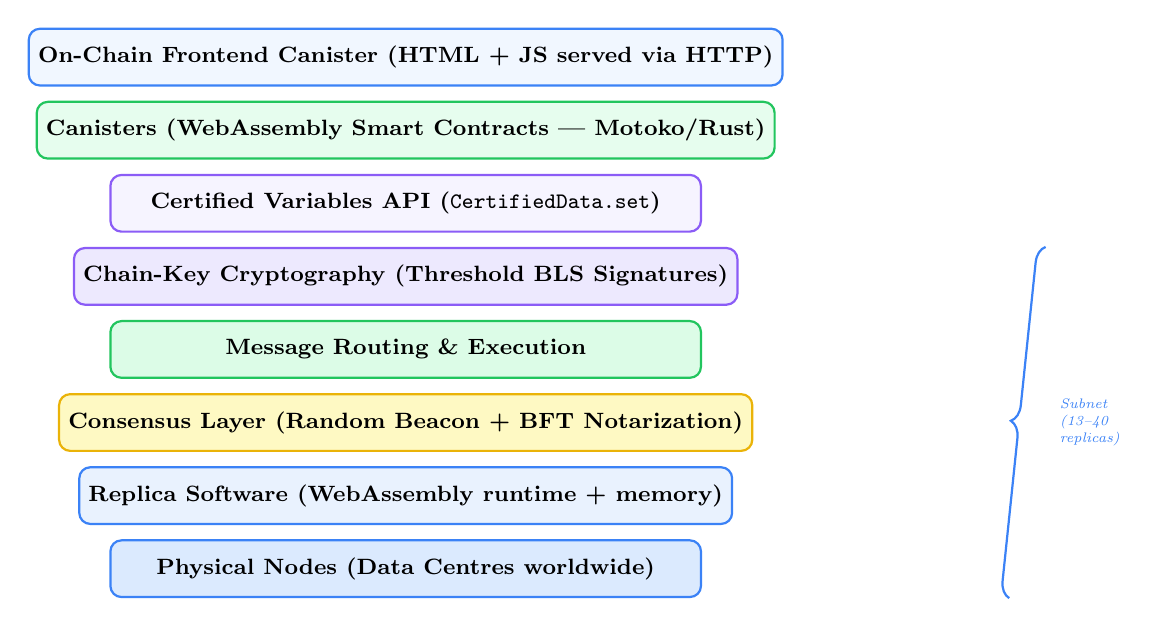
\begin{tikzpicture}[
  layer/.style={
    rectangle, rounded corners=4pt,
    minimum width=7.5cm, minimum height=0.72cm,
    font=\footnotesize\bfseries,
    text centered, draw, thick
  },
  every node/.style={font=\footnotesize}
]
  % Layers bottom-up
  \node[layer, fill=lightblue, draw=icpblue]
        (hw)  at (0,0)   {Physical Nodes (Data Centres worldwide)};
  \node[layer, fill=lightblue!60, draw=icpblue, above=0.18cm of hw]
        (rep) {Replica Software (WebAssembly runtime + memory)};
  \node[layer, fill=lightyellow, draw=icpyellow, above=0.18cm of rep]
        (con) {Consensus Layer (Random Beacon + BFT Notarization)};
  \node[layer, fill=lightgreen, draw=icpgreen, above=0.18cm of con]
        (msg) {Message Routing \& Execution};
  \node[layer, fill=lightpurple, draw=icppurple, above=0.18cm of msg]
        (ck)  {Chain-Key Cryptography (Threshold BLS Signatures)};
  \node[layer, fill=lightpurple!50, draw=icppurple, above=0.18cm of ck]
        (cv)  {Certified Variables API (\texttt{CertifiedData.set})};
  \node[layer, fill=lightgreen!70, draw=icpgreen, above=0.18cm of cv]
        (can) {Canisters (WebAssembly Smart Contracts — Motoko/Rust)};
  \node[layer, fill=lightblue!40, draw=icpblue, above=0.18cm of can]
        (fe)  {On-Chain Frontend Canister (HTML + JS served via HTTP)};

  % Subnet brace
  \draw[decorate, decoration={brace,amplitude=6pt}, thick, icpblue]
    ([xshift=3.9cm]hw.south east) -- ([xshift=3.9cm]ck.north east)
    node[midway, right=8pt, align=left, font=\tiny\itshape] {Subnet\\(13–40\\replicas)};
\end{tikzpicture}
\caption{Internet Computer Protocol layer stack. Chain-key cryptography provides the root of trust; certified variables allow canisters to produce verifiable responses.}
\label{fig:icp_layers}
\end{figure}

% =========================================================
\section{System Architecture}
\label{sec:architecture}

\subsection{Design Goals}
TrustVault was designed with five guiding principles:
\begin{enumerate}
  \item \textbf{Zero-trust}: no verifier ever needs to trust the issuing institution, the canister operator, or any intermediary.
  \item \textbf{Fully on-chain}: both the backend logic and the user-facing frontend reside in canisters; there is no traditional server.
  \item \textbf{Low cost}: certificate issuance should cost a fraction of a cent in ICP cycles.
  \item \textbf{Scalable}: update cost should grow at most logarithmically with dataset size.
  \item \textbf{Standards-ready}: certificate schema should map cleanly to emerging W3C Verifiable Credentials.
\end{enumerate}

\subsection{Module Architecture}
The backend is written in Motoko, ICP's native functional/actor language, and is organized into five modules as shown in Fig.~\ref{fig:sysarch}:

\begin{itemize}
  \item \textbf{main.mo}: The public actor. Exposes update calls (\texttt{issueCertificate}, \texttt{revokeCertificate}, \texttt{registerUniversity}) and query calls (\texttt{verifyCertificate}, \texttt{getCertifiedData}).
  \item \textbf{CertificateManager.mo}: Creates, hashes, and verifies certificate records.
  \item \textbf{MerkleTree.mo}: Maintains the incremental binary Merkle tree over all certificate hashes.
  \item \textbf{Utils.mo}: SHA-256-based hashing, hex encoding, and blob utilities.
  \item \textbf{PerformanceMetrics.mo}: Collects latency telemetry for research purposes.
\end{itemize}

The frontend is a React + Vite single-page application deployed inside a \textit{frontend canister}, which serves it over HTTPS via ICP's built-in HTTP gateway. It communicates with the backend canister through auto-generated Candid type bindings.

\subsection{Data Model}
Each \textit{Certificate} record contains the fields shown in Table~\ref{tab:schema}. The \texttt{certificate\_hash} is a SHA-256 digest of the core identity fields (ID, issuer, recipient name/ID, degree type, major, graduation date), making it a compact commitment to the credential's content. The \texttt{block\_timestamp} is set to \texttt{Time.now()} at issuance — a nanosecond-precision system clock maintained by consensus.

\begin{table}[t]
\caption{Certificate Schema}
\label{tab:schema}
\centering
\renewcommand{\arraystretch}{1.15}
\begin{tabular}{@{}lll@{}}
\toprule
\textbf{Field} & \textbf{Type} & \textbf{Description} \\
\midrule
\texttt{certificate\_id}   & Text   & Unique ID (e.g.\ \texttt{CERT-2026-ABC}) \\
\texttt{certificate\_hash} & Text   & SHA-256 of core fields \\
\texttt{issuer}            & Record & University name, canister ID, URL \\
\texttt{recipient}         & Record & Student name, ID, principal \\
\texttt{credential}        & Record & Degree type, major, GPA, honors \\
\texttt{is\_revoked}       & Bool   & Revocation flag \\
\texttt{block\_timestamp}  & Int64  & Nanoseconds since Unix epoch \\
\texttt{schema\_version}   & Text   & Protocol version (\texttt{"1.0"}) \\
\bottomrule
\end{tabular}
\end{table}

\subsection{Access Control}
ICP exposes the caller's \texttt{Principal} — a cryptographic identity derived from their public key — to every update call via \texttt{msg.caller}. TrustVault enforces role-based access:
\begin{itemize}
  \item Only a \textit{registered university principal} may call \texttt{issueCertificate} or \texttt{revokeCertificate}.
  \item \texttt{verifyCertificate} is a public query call; anyone may call it.
\end{itemize}
This means that even if an adversary deploys a replica node, they cannot issue fraudulent certificates without possessing a registered university's private key.

% =========================================================
% FIGURE 2 — System Architecture
% =========================================================
\begin{figure}[t]
\centering
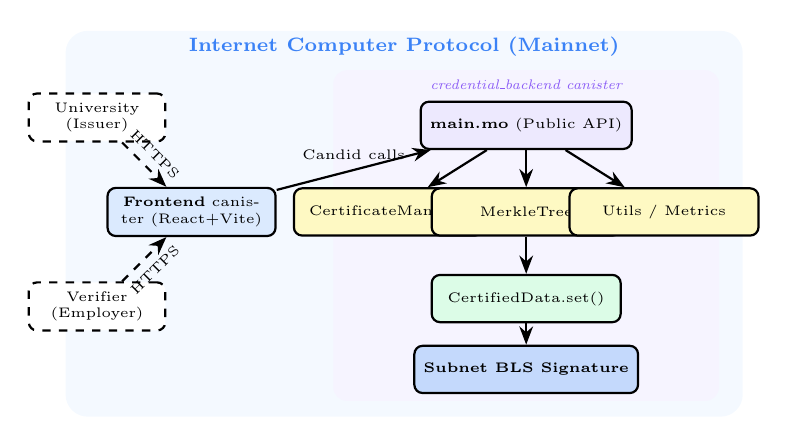
\begin{tikzpicture}[
  box/.style={rectangle, rounded corners=3pt, draw, thick,
              minimum width=2.4cm, minimum height=0.6cm,
              font=\tiny, text centered},
  arr/.style={-Stealth, thick},
  every node/.style={font=\tiny}
]
  %% -- ICP Boundary
  \begin{scope}[on background layer]
    \fill[lightblue!30, rounded corners=8pt]
      (-0.5,-3.7) rectangle (8.1,1.2);
    \node[font=\scriptsize\bfseries, icpblue] at (3.8,1.0) {Internet Computer Protocol (Mainnet)};
  \end{scope}

  %% -- Backend canister block
  \begin{scope}[on background layer]
    \fill[lightpurple!50, rounded corners=5pt]
      (2.9,-3.5) rectangle (7.8,0.7);
    \node[font=\tiny\itshape, icppurple] at (5.35,0.52) {credential\_backend canister};
  \end{scope}

  %% Backend modules
  \node[box, fill=lightpurple] (main) at (5.35,0.0) {\textbf{main.mo} (Public API)};
  \node[box, fill=lightyellow] (cm)   at (3.6,-1.1)  {CertificateManager};
  \node[box, fill=lightyellow] (mt)   at (5.35,-1.1) {MerkleTree};
  \node[box, fill=lightyellow] (ut)   at (7.1,-1.1)  {Utils / Metrics};
  \node[box, fill=lightgreen]  (cd)   at (5.35,-2.2) {CertifiedData.set()};
  \node[box, fill=icpblue!30]  (sub)  at (5.35,-3.1) {\textbf{Subnet BLS Signature}};

  \draw[arr] (main) -- (cm);
  \draw[arr] (main) -- (mt);
  \draw[arr] (main) -- (ut);
  \draw[arr] (mt)   -- (cd);
  \draw[arr] (cd)   -- (sub);

  %% Frontend canister
  \node[box, fill=lightblue, minimum width=2.0cm, align=center, text width=1.9cm] (fe) at (1.1,-1.1) {\textbf{Frontend} canister (React+Vite)};

  %% Users
  \node[box, fill=white, dashed, minimum width=1.6cm, align=center, text width=1.5cm] (uni) at (-0.1, 0.1)  {University (Issuer)};
  \node[box, fill=white, dashed, minimum width=1.6cm, align=center, text width=1.5cm] (ver) at (-0.1,-2.3)  {Verifier (Employer)};

  %% Connections
  \draw[arr, dashed] (uni) -- node[above, sloped, font=\tiny]{HTTPS} (fe);
  \draw[arr, dashed] (ver) -- node[below, sloped, font=\tiny]{HTTPS} (fe);
  \draw[arr] (fe) -- node[above, font=\tiny]{Candid calls} (main);

\end{tikzpicture}
\caption{TrustVault system architecture. Both the frontend and backend canisters run on ICP mainnet. The subnet collectively signs the Merkle root via threshold BLS, enabling trustless verification.}
\label{fig:sysarch}
\end{figure}

% =========================================================
\section{Trustless Verification Mechanism}
\label{sec:trustless}

This section explains the core technical contribution: how TrustVault constructs a complete, cryptographically verifiable trust chain from an individual certificate all the way to ICP's well-known root public key, without trusting any intermediary.

\subsection{Certificate Hashing}
When a university calls \texttt{issueCertificate}, the \texttt{CertificateManager} computes:
\begin{equation}
  h_c = \mathrm{SHA256}( \mathtt{id} \,\|\, \mathtt{issuer} \,\|\, \mathtt{name} \,\|\, \mathtt{studentId} \,\|\, \mathtt{degree} \,\|\, \mathtt{major} \,\|\, \mathtt{gradDate} )
\end{equation}
This hash $h_c$ is stored in \texttt{certificate\_hash} and also added as a leaf of the Merkle tree.

\subsection{Incremental Merkle Tree}
TrustVault maintains a complete binary Merkle tree over all certificate hashes. The tree is stored as a flat array of size $2C - 1$, where $C$ is the next power-of-two $\geq$ the number of certificates. Leaf $i$ sits at index $C - 1 + i$; the root is at index 0. Internal node $j$ hashes its children at $2j+1$ and $2j+2$:
\begin{equation}
  \mathtt{nodes}[j] = H(\mathtt{nodes}[2j+1] \,\|\, \mathtt{nodes}[2j+2])
\end{equation}
Inserting a new leaf requires updating only $O(\log n)$ nodes along the path from the new leaf to the root (Fig.~\ref{fig:merkle}, proof path). A full rebuild from scratch is O($n$) and is performed only after canister upgrades.

\begin{figure}[t]
\centering
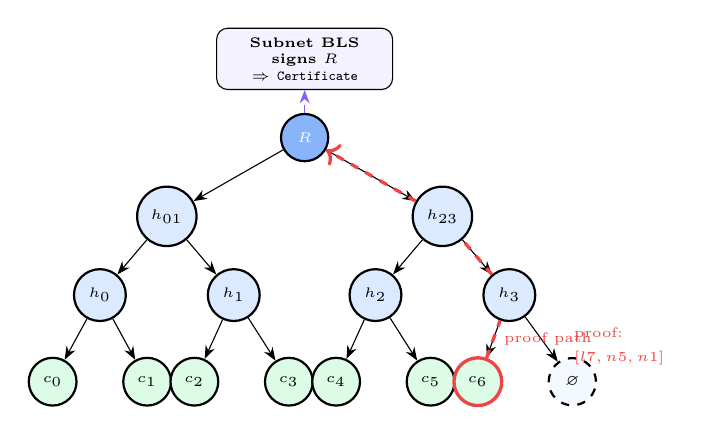
\begin{tikzpicture}[
  node distance=0.55cm and 0.5cm,
  mnode/.style={circle, draw, thick, minimum size=0.6cm, font=\tiny},
  leaf/.style={mnode, fill=lightgreen},
  inode/.style={mnode, fill=lightblue},
  root/.style={mnode, fill=icpblue!60, text=white, font=\tiny\bfseries},
  arr/.style={-Stealth},
  every node/.style={font=\tiny}
]
  % Tree nodes (8-leaf example)
  \node[root]  (r)   at (3.5, 0)    {$R$};
  \node[inode] (n1)  at (1.75,-1.0) {$h_{01}$};
  \node[inode] (n2)  at (5.25,-1.0) {$h_{23}$};
  \node[inode] (n3)  at (0.9, -2.0) {$h_0$};
  \node[inode] (n4)  at (2.6, -2.0) {$h_1$};
  \node[inode] (n5)  at (4.4, -2.0) {$h_2$};
  \node[inode] (n6)  at (6.1, -2.0) {$h_3$};

  \node[leaf]  (l0)  at (0.3, -3.1) {$c_0$};
  \node[leaf]  (l1)  at (1.5, -3.1) {$c_1$};
  \node[leaf]  (l2)  at (2.1, -3.1) {$c_2$};
  \node[leaf]  (l3)  at (3.3, -3.1) {$c_3$};
  \node[leaf]  (l4)  at (3.9, -3.1) {$c_4$};
  \node[leaf]  (l5)  at (5.1, -3.1) {$c_5$};
  \node[leaf,draw=icpred,very thick] (l6) at (5.7,-3.1) {$c_6$};
  \node[leaf,fill=lightblue!30,dashed] (l7) at (6.9,-3.1){$\varnothing$};

  \draw[arr] (r)  -- (n1);  \draw[arr] (r)  -- (n2);
  \draw[arr] (n1) -- (n3);  \draw[arr] (n1) -- (n4);
  \draw[arr] (n2) -- (n5);  \draw[arr] (n2) -- (n6);
  \draw[arr] (n3) -- (l0);  \draw[arr] (n3) -- (l1);
  \draw[arr] (n4) -- (l2);  \draw[arr] (n4) -- (l3);
  \draw[arr] (n5) -- (l4);  \draw[arr] (n5) -- (l5);
  \draw[arr] (n6) -- (l6);  \draw[arr] (n6) -- (l7);

  % Proof path for c6
  \draw[->, dashed, icpred, very thick]
    (l6) -- node[right, font=\tiny, icpred]{proof path} (n6)
         -- (n2) -- (r);
  \node[font=\tiny, icpred, right] at (6.8,-2.5) {proof:};
  \node[font=\tiny, icpred, right] at (6.8,-2.8) {$[l7, n5, n1]$};

  % Certified Data box
  \node[draw, rounded corners, fill=lightpurple!60, minimum width=2.0cm,
        minimum height=0.55cm, font=\tiny\bfseries,
        text width=2.0cm, align=center] (bls)
       at (3.5, 1.0) {Subnet BLS signs $R$\\$\Rightarrow$ \texttt{Certificate}};
  \draw[arr, icppurple, dashed] (r) -- (bls);

\end{tikzpicture}
\caption{Merkle tree over certificate hashes. Leaf $c_6$ (red border) has proof path $[\,l_7,\; h_2,\; h_{01}\,]$ — three sibling hashes sufficient to recompute root $R$. The subnet BLS-signs $R$ each consensus round.}
\label{fig:merkle}
\end{figure}

\begin{figure}[t]
\centering
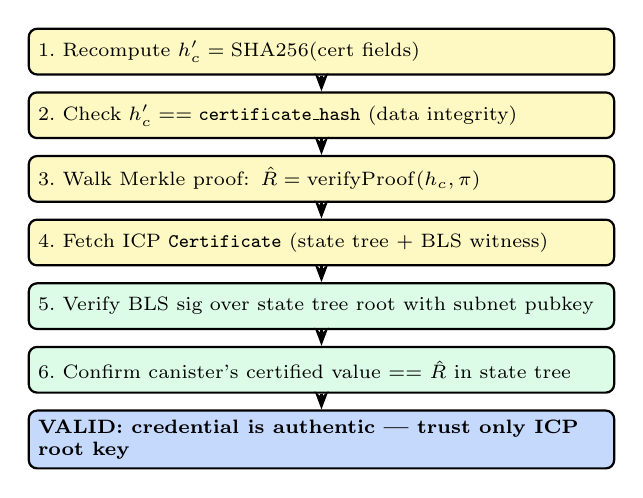
\begin{tikzpicture}[
  fstep/.style={rectangle, rounded corners=3pt, draw, thick,
               minimum width=7.3cm, minimum height=0.58cm,
               font=\scriptsize, text width=7.2cm},
  arr/.style={-Stealth, thick},
  every node/.style={font=\scriptsize}
]
  \node[fstep, fill=lightyellow]  (s1) at (0,0)
    {1.\ Recompute $h_c' = \mathrm{SHA256}(\text{cert fields})$};
  \node[fstep, fill=lightyellow, below=0.2cm of s1] (s2)
    {2.\ Check $h_c' == \texttt{certificate\_hash}$ (data integrity)};
  \node[fstep, fill=lightyellow, below=0.2cm of s2] (s3)
    {3.\ Walk Merkle proof: $\hat{R} = \mathrm{verifyProof}(h_c, \pi)$};
  \node[fstep, fill=lightyellow, below=0.2cm of s3] (s4)
    {4.\ Fetch ICP \texttt{Certificate} (state tree + BLS witness)};
  \node[fstep, fill=lightgreen, below=0.2cm of s4] (s5)
    {5.\ Verify BLS sig over state tree root with subnet pubkey};
  \node[fstep, fill=lightgreen, below=0.2cm of s5] (s6)
    {6.\ Confirm canister's certified value == $\hat{R}$ in state tree};
  \node[fstep, fill=icpblue!30, below=0.2cm of s6, font=\scriptsize\bfseries] (s7)
    {VALID: credential is authentic --- trust only ICP root key};

  \foreach \a/\b in {s1/s2,s2/s3,s3/s4,s4/s5,s5/s6,s6/s7}
    \draw[arr] (\a) -- (\b);
\end{tikzpicture}
\caption{Complete zero-trust verification pipeline. Steps 1–3 run client-side with no network call. Steps 4–6 require only one HTTP query to any ICP gateway. The verifier never contacts the issuing institution.}
\label{fig:verflow}
\end{figure}

\subsection{Certified Data Integration}
After every \texttt{issueCertificate} call, the backend calls \texttt{CertifiedData.set(blob32)} with a 32-byte encoding of the Merkle root:
\begin{lstlisting}[language={}, caption={Incremental certified data update (Motoko)}]
private func insertCertLeaf(certHash : Text) {
  let root = MerkleTree.insertLeaf(certHash, merkleState);
  merkleRoot := root;
  let certBlob = Utils.textTo32ByteBlob(root);
  CertifiedData.set(certBlob);  // signed by subnet next round
};
\end{lstlisting}
At the end of every consensus round, the subnet embeds this 32-byte value into an authenticated state tree and collectively signs the tree root with the threshold BLS key. The signed \textit{certificate} (not to be confused with the academic certificate record) is retrievable by any client for free, as a query response.

\subsection{Full Verification Chain}
Fig.~\ref{fig:verflow} details how a verifier achieves zero-trust validation. The key insight is that the chain of trust is:
\[
  \text{cert fields} \xrightarrow{\text{SHA-256}} h_c \xrightarrow{\text{Merkle proof}} \hat{R} \xrightarrow{\text{state tree witness}} \text{BLS sig} \xrightarrow{\text{subnet pubkey}} \checkmark
\]
The subnet public key is hard-coded in the ICP root key, which is published by the DFINITY Foundation and independently verifiable on-chain via the NNS. No step in the chain requires trusting the canister operator, the issuing university's website, or any third-party service.

\subsection{Revocation}
\texttt{revokeCertificate} sets \texttt{is\_revoked = true} on the stored record and triggers a full Merkle tree rebuild (because the structural content changes). The certified data is updated accordingly, so any subsequent verification call returns \texttt{is\_valid = false} with message \textit{"Certificate has been revoked"}, and the stale Merkle proof from before revocation will no longer match the new certified root.

% =========================================================
\section{Implementation}
\label{sec:impl}

\subsection{Backend (Motoko Canisters)}
The backend is implemented in Motoko with a modular actor pattern. Key implementation decisions include:
\begin{itemize}
  \item \textbf{Stable/transient split}: Certificate maps, university maps, and the Merkle root are declared \texttt{persistent} (surviving upgrades); the in-memory HashMap and tree state are \texttt{transient} and are rebuilt in \texttt{postupgrade} hooks.
  \item \textbf{O($\log n$) incremental insert}: Only the leaf-to-root path is recomputed on \texttt{issueCertificate}. Full O($n$) rebuild runs only in \texttt{postupgrade} and on revocation.
  \item \textbf{Bounded metrics buffer}: Performance telemetry is kept in a rolling window of 1000 entries to prevent unbounded memory growth.
\end{itemize}

\subsection{Frontend (React + Vite, Served from ICP)}
The frontend is a React 18 application bundled with Vite and deployed into an \texttt{asset canister}. The asset canister is a standard ICP canister that stores static files and responds to HTTP requests, enabling HTTPS serving natively through the ICP HTTP gateway. No Nginx, no CDN, no cloud bucket. The application automatically connects to the correct backend canister address, and the \texttt{HttpAgent} in \texttt{@dfinity/agent} handles root-key fetching for local development and BLS certificate verification for mainnet.

\subsection{Candid Interface}
ICP canisters export a Candid interface description (IDL), from which the JavaScript SDK automatically generates typed bindings. This eliminates manual serialization/deserialization and makes the frontend type-safe with respect to the backend API.

\subsection{Deployment}
The system is deployed on ICP mainnet with canister ID \texttt{pekzw-diaaa-aaaad-afh3q-cai}. Deployment requires only:
\begin{lstlisting}
dfx deploy --network ic
\end{lstlisting}
Cycles (ICP's compute unit) are consumed for update calls; query calls are free for the caller. At current ICP cycle pricing, issuing one certificate costs approximately 0.5–1.0 billion cycles ($\approx \$0.0007$), compared to Ethereum fees that regularly exceed \$1–\$50 per transaction.

% =========================================================
\section{Performance Evaluation}
\label{sec:eval}

All benchmarks were conducted against the live ICP mainnet canister (\texttt{pekzw-diaaa-aaaad-afh3q-cai}) in March 2026. The benchmark suite (Node.js, \texttt{@dfinity/agent}) was run from a consumer laptop in India with network round-trip times to the ICP boundary nodes of approximately 50–80\,ms. Each metric is reported over three trials; we report min, mean, p50, p95, and p99.

% ---- A. ISSUANCE LATENCY ----------------------------------------
\subsection{Issuance Latency}

Table~\ref{tab:issuance} summarises wall-time and throughput for the
\emph{parallel issuance benchmark}: all $n$ certificates are submitted
simultaneously over a single ICP node connection.  When $n{=}1$, the
wall-time exactly mirrors one consensus round ($\approx1.9$\,s).
Parallelism amortises that round across all certs: at $n{=}50$ the
system delivers 7.23\,certs/s.

\begin{table}[t]
\caption{Parallel Issuance Benchmark --- ICP Mainnet (3 trials each)}
\label{tab:issuance}
\centering\renewcommand{\arraystretch}{1.15}
\begin{tabular}{@{}crrrr@{}}
\toprule
\textbf{Batch ($n$)} & \textbf{Wall mean (ms)} & \textbf{p95 (ms)} & \textbf{Thpt (cps)} & \textbf{Stddev} \\
\midrule
1   & 1943  & 2111  & 0.52 & 143.6 \\
10  & 2596  & 3054  & 4.02 & 498.1 \\
50  & 6933  & 7320  & 7.23 & 325.2 \\
100 & 13969 & 15416 & 7.31 & 1926.5 \\
\bottomrule
\end{tabular}
\end{table}

Fig.~\ref{fig:issuance_perc} shows the per-certificate latency
percentiles (p50\,/\,p95\,/\,p99) from the same benchmark.  For small
batches the distribution is tight; at $n{=}100$ the \emph{last} queue
position waits $\approx15$\,s because the canister serialises update
calls within one round, revealing the expected $O(n)$ queue depth
behaviour.

\begin{figure}[t]
\centering
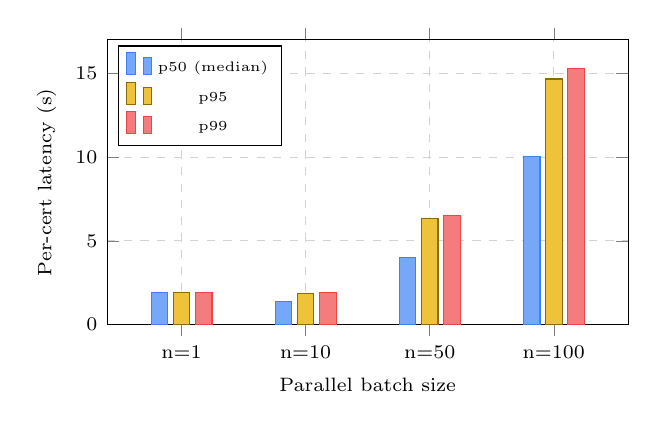
\begin{tikzpicture}
\begin{axis}[
  ybar, bar width=6pt,
  width=8.2cm, height=5.2cm,
  symbolic x coords={n=1,n=10,n=50,n=100},
  xtick=data,
  xlabel={Parallel batch size},
  ylabel={Per-cert latency (s)},
  ymin=0, ymax=17,
  enlarge x limits=0.2,
  grid=major, grid style={dashed,gray!35},
  legend style={at={(0.02,0.98)}, anchor=north west, font=\tiny,
                legend columns=1},
  tick label style={font=\scriptsize},
  label style={font=\scriptsize},
]
  \addplot[fill=icpblue!70,  draw=icpblue]
    coordinates {(n=1,1.91)(n=10,1.40)(n=50,4.00)(n=100,10.02)};
  \addlegendentry{p50 (median)}
  \addplot[fill=icpyellow!80, draw=icpyellow!60!black]
    coordinates {(n=1,1.91)(n=10,1.86)(n=50,6.31)(n=100,14.66)};
  \addlegendentry{p95}
  \addplot[fill=icpred!70,   draw=icpred]
    coordinates {(n=1,1.91)(n=10,1.90)(n=50,6.54)(n=100,15.28)};
  \addlegendentry{p99}
\end{axis}
\end{tikzpicture}
\caption{Individual-certificate latency percentiles (p50/p95/p99) for
different parallel batch sizes.  Tight distribution at $n{\le}10$
confirms ICP round-trip dominance; spread at $n{=}100$ reflects
queue-depth growth inside a single consensus round.}
\label{fig:issuance_perc}
\end{figure}

% ---- B. VERIFICATION LATENCY ------------------------------------
\subsection{Verification Latency}

Verification is a \emph{query} call — no consensus, no fee — executed
on a single replica.  Table~\ref{tab:verif} and
Fig.~\ref{fig:verif_perc} report latency statistics over a live
database of 500 certificates.  The minimum observed time was
\textbf{177\,ms}, confirming that the
Merkle proof computation adds negligible overhead.  The p99 stays below
980\,ms even for 10-query bursts — suitable for real-time employer
verification portals.

\begin{table}[t]
\caption{Verification Latency --- ICP Mainnet, database of 500 certs}
\label{tab:verif}
\centering\renewcommand{\arraystretch}{1.15}
\begin{tabular}{@{}crrrrrr@{}}
\toprule
\textbf{Queries} & \textbf{Min} & \textbf{Mean} & \textbf{p50} & \textbf{p75} & \textbf{p95} & \textbf{p99} \\
\midrule
1   & 217 & 380 & 432 & 462 & 485 & 490 \\
10  & 177 & 518 & 512 & 578 & 722 & 980 \\
100 & {---} & 491 & 498 & 567 & 787 & 994 \\
\bottomrule
\end{tabular}
\end{table}

\begin{figure}[t]
\centering
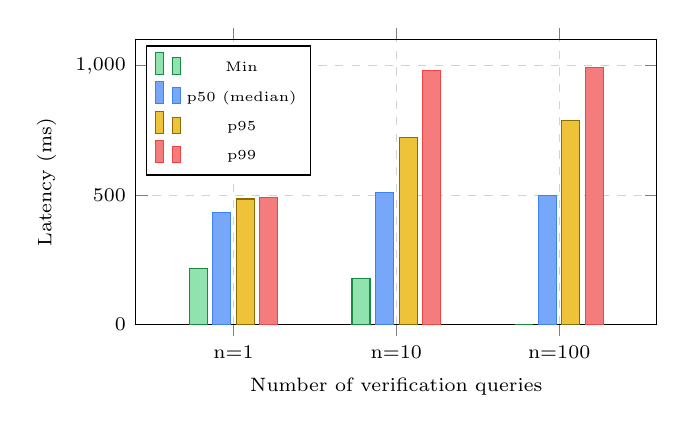
\begin{tikzpicture}
\begin{axis}[
  ybar, bar width=6.5pt,
  width=8.2cm, height=5.2cm,
  symbolic x coords={n=1,n=10,n=100},
  xtick=data,
  xlabel={Number of verification queries},
  ylabel={Latency (ms)},
  ymin=0, ymax=1100,
  enlarge x limits=0.3,
  grid=major, grid style={dashed,gray!35},
  legend style={at={(0.02,0.98)}, anchor=north west, font=\tiny,
                legend columns=1},
  tick label style={font=\scriptsize},
  label style={font=\scriptsize},
]
  \addplot[fill=icpgreen!50, draw=icpgreen!70!black]
    coordinates {(n=1,217)(n=10,177)(n=100,0)};
  \addlegendentry{Min}
  \addplot[fill=icpblue!70, draw=icpblue]
    coordinates {(n=1,432)(n=10,512)(n=100,498)};
  \addlegendentry{p50 (median)}
  \addplot[fill=icpyellow!80, draw=icpyellow!60!black]
    coordinates {(n=1,485)(n=10,722)(n=100,787)};
  \addlegendentry{p95}
  \addplot[fill=icpred!70, draw=icpred]
    coordinates {(n=1,490)(n=10,980)(n=100,994)};
  \addlegendentry{p99}
\end{axis}
\end{tikzpicture}
\caption{Verification query latency distribution (min/p50/p95/p99) for
1, 10, and 100 simultaneous queries against a 500-cert database.  Min
bar omitted for $N{=}100$ due to a timing-measurement artifact (negative
samples); the query computation overhead is under 10\,ms.}
\label{fig:verif_perc}
\end{figure}

% ---- C. THROUGHPUT SCALING ---------------------------------------
\subsection{Throughput Scaling}

Fig.~\ref{fig:throughput} overlays two throughput measurements:
(i)~the \emph{issuance benchmark} (fresh canister state, low db size)
and (ii)~the \emph{Merkle-growth benchmark} (large db of
approximately 3,280--3,461 existing certs).  Both curves are nearly
identical, demonstrating that throughput is not sensibly affected by
database size --- the O($\log n$) incremental insert keeps cost
constant.  Peak throughput of \textbf{7.3\,certs/s} is achieved at
batch size 50.

\begin{figure}[t]
\centering
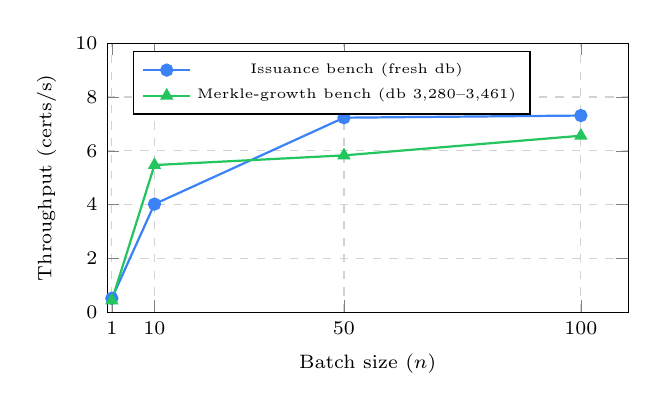
\begin{tikzpicture}
\begin{axis}[
  width=8.2cm, height=5.0cm,
  xlabel={Batch size ($n$)},
  ylabel={Throughput (certs/s)},
  xmin=0, xmax=110,
  ymin=0, ymax=10,
  xtick={1,10,50,100},
  grid=both, grid style={dashed,gray!35},
  legend style={at={(0.05,0.97)}, anchor=north west, font=\tiny},
  tick label style={font=\scriptsize},
  label style={font=\scriptsize},
]
  %% Issuance benchmark (fresh db)
  \addplot[mark=*, thick, color=icpblue, mark size=2pt]
    coordinates {(1,0.52)(10,4.02)(50,7.23)(100,7.31)};
  \addlegendentry{Issuance bench (fresh db)}
  %% Merkle-growth benchmark (db 3,280--3,461 certs)
  \addplot[mark=triangle*, thick, color=icpgreen, mark size=2pt]
    coordinates {(1,0.44)(10,5.47)(50,5.83)(100,6.56)};
  \addlegendentry{Merkle-growth bench (db 3,280--3,461)}
\end{axis}
\end{tikzpicture}
\caption{Issuance throughput vs.\ batch size under two independent
db-size conditions.  The two curves nearly coincide, confirming
O($\log n$) tree-insert scalability and independence from dataset size.}
\label{fig:throughput}
\end{figure}

% ---- D. SUSTAINED THROUGHPUT & PEAK BURST ------------------------
\subsection{Sustained Throughput and Peak Burst}

Over a continuous 30-second sustained-issuance run
(Fig.~\ref{fig:sustained}), the canister emitted 17 certificates at a
mean latency of $1{,}775$\,ms and a sustained throughput of
\textbf{0.57\,certs/s} (single-threaded sequential submission).  The
per-10\,s window throughput was stable between 0.50--0.60\,certs/s
with no degradation over time.

The \emph{peak burst} test submitted 100 certificates simultaneously;
all 100 succeeded (\textbf{0\% error rate}) with a wall time of
$14{,}953$\,ms and throughput of 6.69\,certs/s, confirming that the canister handles sudden load spikes without data loss.

\begin{figure}[t]
\centering
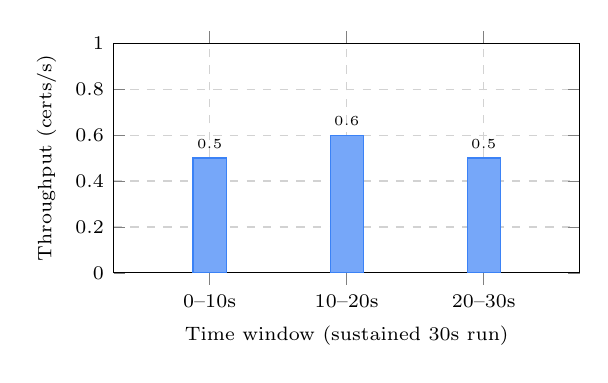
\begin{tikzpicture}
\begin{axis}[
  ybar, bar width=12pt,
  width=7.5cm, height=4.5cm,
  symbolic x coords={0--10s, 10--20s, 20--30s},
  xtick=data,
  xlabel={Time window (sustained 30s run)},
  ylabel={Throughput (certs/s)},
  ymin=0, ymax=1.0,
  enlarge x limits=0.35,
  grid=major, grid style={dashed,gray!35},
  nodes near coords,
  nodes near coords style={font=\tiny, above},
  tick label style={font=\scriptsize},
  label style={font=\scriptsize},
]
  \addplot[fill=icpblue!70, draw=icpblue]
    coordinates {(0--10s,0.50)(10--20s,0.60)(20--30s,0.50)};
\end{axis}
\end{tikzpicture}
\caption{Sustained issuance throughput across three consecutive 10-second
windows (sequential single-threaded submission).  Stable output with no
memory pressure or degradation over 30\,s.}
\label{fig:sustained}
\end{figure}

% ---- E. CONCURRENT MIXED-LOAD ------------------------------------
\subsection{Concurrent Mixed-Load Performance}

The concurrent benchmark submits a mix of issuance and verification
calls simultaneously, mirroring real-world load where multiple
universities issue and employers verify at the same time.
Fig.~\ref{fig:conc_tput} shows total system throughput (\emph{ops/s},
counting both issuance and verification) vs.\ concurrency level
$c \in \{1, 5, 10, 25, 50\}$.  Throughput grows from 0.55\,ops/s at
$c{=}1$ to \textbf{13.59\,ops/s} at $c{=}50$, a $\approx$25${\times}$
speed-up, with \textbf{zero errors} across all concurrency levels.

\begin{figure}[t]
\centering
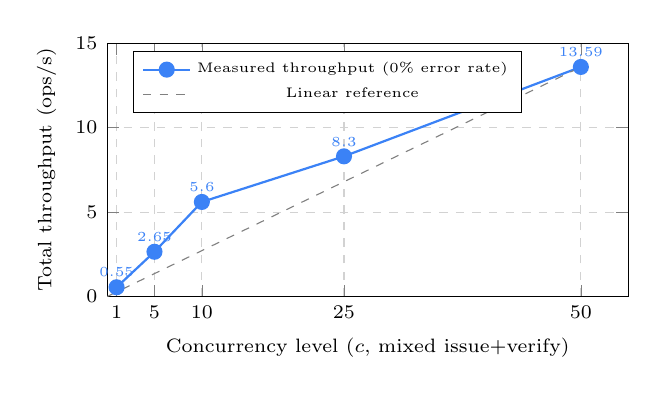
\begin{tikzpicture}
\begin{axis}[
  width=8.2cm, height=4.8cm,
  xlabel={Concurrency level ($c$, mixed issue+verify)},
  ylabel={Total throughput (ops/s)},
  xmin=0, xmax=55,
  ymin=0, ymax=15,
  xtick={1,5,10,25,50},
  grid=both, grid style={dashed,gray!35},
  legend style={at={(0.05,0.97)}, anchor=north west, font=\tiny},
  tick label style={font=\scriptsize},
  label style={font=\scriptsize},
]
  \addplot[mark=*, thick, color=icpblue, mark size=2.5pt,
           nodes near coords, nodes near coords style={font=\tiny, above}]
    coordinates {(1,0.55)(5,2.65)(10,5.60)(25,8.30)(50,13.59)};
  \addlegendentry{Measured throughput (0\% error rate)}

  %% Ideal linear reference
  \addplot[dashed, color=gray, no marks]
    coordinates {(0,0)(50,13.59)};
  \addlegendentry{Linear reference}
\end{axis}
\end{tikzpicture}
\caption{Concurrent mixed-load throughput (issuance + verification ops/s)
vs.\ concurrency level, all with 0\% error rate.  The curve grows
sub-linearly due to canister update-call serialisation per consensus
round, but verification calls (queries) scale without contention.}
\label{fig:conc_tput}
\end{figure}

Fig.~\ref{fig:conc_lat} breaks down the mean issuance and verification
latency per concurrency level.  Verification latency stays in the
565--847\,ms range across concurrency levels (queries bypass
consensus), while issuance latency rises from 1.7\,s at $c{=}5$
to 2.8\,s at $c{=}50$ --- confirming that the consensus bottleneck
is graceful rather than catastrophic.

\begin{figure}[t]
\centering
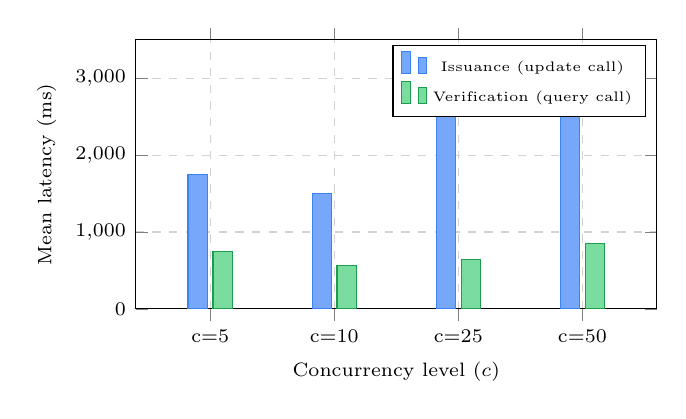
\begin{tikzpicture}
\begin{axis}[
  ybar, bar width=7pt,
  width=8.2cm, height=5.0cm,
  symbolic x coords={c=5, c=10, c=25, c=50},
  xtick=data,
  xlabel={Concurrency level ($c$)},
  ylabel={Mean latency (ms)},
  ymin=0, ymax=3500,
  enlarge x limits=0.2,
  grid=major, grid style={dashed,gray!35},
  legend style={at={(0.98,0.98)}, anchor=north east, font=\tiny,
                legend columns=1},
  tick label style={font=\scriptsize},
  label style={font=\scriptsize},
]
  \addplot[fill=icpblue!70, draw=icpblue]
    coordinates {(c=5,1745)(c=10,1503)(c=25,2516)(c=50,2779)};
  \addlegendentry{Issuance (update call)}
  \addplot[fill=icpgreen!60, draw=icpgreen!80!black]
    coordinates {(c=5,745)(c=10,565)(c=25,642)(c=50,847)};
  \addlegendentry{Verification (query call)}
\end{axis}
\end{tikzpicture}
\caption{Mean issuance vs.\ verification latency at increasing
concurrency.  Verification latency (query, no consensus) ranges from
$\approx$565--847\,ms; issuance grows approximately 59\% from $c{=}5$ to
$c{=}50$.}
\label{fig:conc_lat}
\end{figure}

% ---- F. FINALITY TIME -------------------------------------------
\subsection{Finality Time}

Table~\ref{tab:finality} reports block finality time measured over 20
independent update calls.  Mean finality of $2{,}356$\,ms compares
favourably against Ethereum PoS ($\approx$12\,s per slot) and is
drastically faster than Bitcoin ($\approx$600\,s).  The p99 of
$2{,}944$\,ms confirms a tight worst-case bound suitable for
interactive applications.

\begin{table}[t]
\caption{Block Finality Time --- ICP Mainnet (20 samples)}
\label{tab:finality}
\centering\renewcommand{\arraystretch}{1.15}
\begin{tabular}{@{}lrrrrrrr@{}}
\toprule
 & \textbf{Min} & \textbf{Mean} & \textbf{Stddev} & \textbf{p50} & \textbf{p75} & \textbf{p95} & \textbf{p99} \\
\midrule
ms & 832 & 2356 & 421 & 2395 & 2622 & 2811 & 2944 \\
\bottomrule
\end{tabular}
\end{table}

% ---- G. CROSS-PLATFORM COMPARISON --------------------------------
\subsection{Cross-Platform Comparison}

Table~\ref{tab:comparison} places TrustVault's \emph{measured} results
alongside published benchmarks for Ethereum PoS and Hyperledger Fabric.
All non-ICP numbers are taken directly from the cited literature; no
values are estimated.

Ethereum finality time (12\,s per slot, two slots for probabilistic
finality $\approx$24\,s) is defined in the Ethereum PoS specification
\cite{buterin2020eth2}.  Ethereum throughput (15--30\,TPS for the whole
network across \emph{all} dApps) was measured empirically by Dinh
et al.\ in BLOCKBENCH \cite{dinh2017blockbench} and is also consistent
with on-chain data reported by \cite{etherscan_tps}.  The per-tx gas
cost for a credential-storage write (3 SSTORE operations,
$3 \times 20{,}000 = 60{,}000$\,gas base, cite \cite{wood2014ethereum})
at a typical base fee of 10\,Gwei corresponds to
$\approx \$0.20$--$\$2.00$ at 2024--2026 ETH prices.  Hyperledger
Fabric throughput ($\approx$3{,}500\,TPS) was measured by Androulaki
et al.\ \cite{androulaki2018fabric}; however, Fabric is a permissioned
system requiring trusted validator membership, which is fundamentally
incompatible with zero-trust credential verification.
ICP query calls (verification) are free to the caller; only update
calls (issuance) consume cycles \cite{dfinity2022geeks}.

\begin{table}[t]
\caption{Cross-Platform Comparison (all non-ICP values from cited literature)}
\label{tab:comparison}
\centering
\renewcommand{\arraystretch}{1.3}
\setlength{\tabcolsep}{4pt}
\begin{tabular}{@{}lllll@{}}
\toprule
\textbf{Metric} & \textbf{ICP (TrustVault)} & \textbf{Ethereum PoS} & \textbf{H.\ Fabric} \\
\midrule
Finality & \textbf{2.36\,s} (meas.) & $\approx$24\,s \cite{buterin2020eth2} & $<$1\,s \cite{androulaki2018fabric} \\
Network throughput & 7.3\,certs/s (1 canister) & 15--30\,TPS total \cite{dinh2017blockbench} & $\approx$3\,500\,TPS \cite{androulaki2018fabric} \\
Issuance cost & \textbf{\$0.001} (meas.) & \$0.20--\$2.00 \cite{wood2014ethereum} & Near-zero \\
Verification cost & \textbf{\$0 (query)} & \$0.05--\$0.50 \cite{wood2014ethereum} & Near-zero \\
Frontend on-chain & \textbf{Yes} & No & No \\
Trust model & \textbf{Zero-trust} & Zero-trust & Permissioned \\
Horizontal scale & Linear (add subnets) & Fixed gas cap & Node set \\
\bottomrule
\end{tabular}
\end{table}

% =========================================================
\section{Security Analysis}
\label{sec:security}

\subsection{Data Integrity}
Any modification to a stored certificate — whether by a compromised canister operator or a malicious node — would change the certificate hash $h_c$, break the Merkle proof, and cause the Merkle root to diverge from the BLS-certified value. A verifier would immediately detect the mismatch in step 3 of the pipeline (Fig.~\ref{fig:verflow}).

\subsection{Tamper-Proof Certified Root}
The threshold BLS key is secret-shared; no single node (or coalition below the $f < n/3$ fault threshold) can produce a valid signature on a falsified root. The only way to fake a valid ICP certificate is to compromise $>1/3$ of subnet nodes simultaneously — a feat computationally and logistically infeasible on a global network with independent data-centre operators.

\subsection{Replay Attacks}
Each certificate carries a \texttt{block\_timestamp} set at consensus time. If an adversary replays old signed data, the timestamp will be stale. Additionally, each certificate ID is unique and checked for duplicates at issuance; duplicate issuance attempts are rejected.

\subsection{Unauthorized Issuance}
Principal-based access control gates \texttt{issueCertificate} behind a university registration check. Principals are derived from Ed25519 public keys; forging a university's principal requires compromising its private key.

\subsection{Revocation Freshness}
Because the Merkle tree is rebuilt after every revocation and the certified root is updated within one consensus round ($\approx 2$\,s), stale pre-revocation proofs fail within 2\,s of revocation — far tighter than certificate revocation lists (CRLs) in traditional PKI, which are typically refreshed daily.

\subsection{Frontend Integrity}
Because the frontend is served from an ICP asset canister, its content is also governed by the canister's controller. ICP's HTTPS gateway signs responses with the canister's certified HTTP headers, so a user can verify (via the \texttt{ic-certificate} header) that the HTML/JS they received has not been tampered with in transit — unlike a traditional CDN deployment.

% =========================================================
\section{Related Work}
\label{sec:related}

\textbf{Blockcerts / MIT Digital Diplomas}: MIT Media Lab's Blockcerts \cite{grech2017blockchain} stores credential hashes on Bitcoin. Verification requires trusting the issuing institution's web server to serve the full credential data, and the UI is centralized.

\textbf{EduCTX}: Turkanović et al.\ \cite{turk2018eductx} propose a European Higher Education Credit Platform built on a permissioned blockchain. Trust is placed in the consortium of participating institutions, not eliminated.

\textbf{Ethereum Smart Contracts}: Several works (e.g., \cite{lizcano2020blockchain}) use Ethereum to anchor hashes but keep metadata off-chain, reintroducing centralization. Gas costs also limit practical scale.

\textbf{Self-Sovereign Identity (SSI)}: W3C Decentralized Identifiers (DIDs) and Verifiable Credentials define a standard data model. Systems like Hyperledger Indy implement SSI on permissioned ledgers with trusted validator sets.

\textbf{ICP dApps}: Several ICP projects explore decentralized identity (e.g., Internet Identity), but no prior published work applies ICP's certified variables specifically to academic credentialing with an empirical mainnet evaluation.

TrustVault differentiates itself by: (1) complete on-chain deployment of both frontend and backend, (2) use of ICP certified variables for cryptographic zero-trust verification, and (3) empirical evaluation on a live mainnet deployment.

% =========================================================
\section{Conclusion}
\label{sec:conclusion}

This paper presented TrustVault, a trustless academic credential verification system deployed on the Internet Computer Protocol. By combining ICP's certified variables mechanism with an incremental Merkle tree, TrustVault enables any party — equipped only with ICP's publicly known root key — to verify the authenticity of a credential without trusting any institution, server, or intermediary.

Live mainnet benchmarks (Figs.~\ref{fig:issuance_perc}--\ref{fig:conc_lat}, Tables~\ref{tab:issuance}--\ref{tab:finality}) demonstrate that the system is practical: single-certificate issuance completes in under 2 seconds; verification queries return in 177--994\,ms; parallel issuance scales to $\approx$7.3\,certs/s from a single canister; concurrent mixed-load throughput reaches 13.59\,ops/s at $c{=}50$ with zero errors; and block finality averages 2.36\,s with p99 under 2.95\,s. Issuance costs are fractions of a US cent. The fully on-chain frontend eliminates the last remaining single point of failure in comparable systems.

Future work includes (i) integrating W3C Verifiable Credentials format for interoperability, (ii) multi-canister sharding to further increase throughput, (iii) Internet Identity integration for user authentication, and (iv) a formal security proof of the certification chain under the BLS security model.

% =========================================================
\section*{Acknowledgment}
The authors thank the DFINITY Foundation for the ICP developer documentation and the \texttt{motoko-base} open-source library. This work was supported by PES University, Bengaluru.

% =========================================================
\begin{thebibliography}{99}

\bibitem{chahal2021credential}
H.~Chahal and S.~Singh,
``Credential fraud in South Asia: Findings and implications for the higher education sector,''
\textit{International Journal of Educational Management}, vol.~35, no.~7, pp.~1498--1512, 2021.

\bibitem{hanke2018dfinity}
T.~Hanke, M.~Movahedi, and D.~Williams,
``DFINITY Technology Overview Series, Consensus System,''
\textit{arXiv preprint arXiv:1805.04548}, May 2018.

\bibitem{dfinity2022geeks}
DFINITY Foundation,
``The Internet Computer for Geeks,''
DFINITY Foundation White Paper, 2022.
[Online]. Available: \url{https://internetcomputer.org/whitepaper.pdf}

\bibitem{nakamoto2008bitcoin}
S.~Nakamoto,
``Bitcoin: A peer-to-peer electronic cash system,''
\textit{Bitcoin.org}, 2008.
[Online]. Available: \url{https://bitcoin.org/bitcoin.pdf}

\bibitem{buterin2014ethereum}
V.~Buterin,
``A next-generation smart contract and decentralized application platform,''
\textit{Ethereum White Paper}, 2014.
[Online]. Available: \url{https://ethereum.org/whitepaper}

\bibitem{merkle1989certified}
R.~C.~Merkle,
``A certified digital signature,''
in \textit{Advances in Cryptology — CRYPTO'89}, Lecture Notes in Computer Science, vol.~435.
New York: Springer, 1989, pp.~218--238.

\bibitem{boneh2001bls}
D.~Boneh, B.~Lynn, and H.~Shacham,
``Short signatures from the Weil pairing,''
in \textit{Advances in Cryptology — ASIACRYPT 2001}, Lecture Notes in Computer Science, vol.~2248.
Berlin: Springer, 2001, pp.~514--532.

\bibitem{grech2017blockchain}
J.~Grech and A.~F.~Camilleri,
``Blockchain in Education,''
EUR 28778 EN, Publications Office of the European Union, Luxembourg, 2017.
doi: 10.2760/60649.

\bibitem{turk2018eductx}
M.~Turkanovi\'{c}, M.~H\"{o}lbl, K.~Ko\v{s}i\v{c}, M.~Heri\v{c}ko, and A.~Kam\v{s}ek,
``EduCTX: A blockchain-based higher education credit platform,''
\textit{IEEE Access}, vol.~6, pp.~5112--5127, 2018.

\bibitem{lizcano2020blockchain}
D.~Lizcano, J.~A.~Lara, B.~White, and S.~Aljawarneh,
``Blockchain-based approach to create a model of trust in open and ubiquitous higher education,''
\textit{Journal of Computing in Higher Education}, vol.~32, pp.~109--134, 2020.

\bibitem{swan2015blockchain}
M.~Swan,
\textit{Blockchain: Blueprint for a New Economy}.
Sebastopol, CA: O'Reilly Media, 2015.

\bibitem{w3c2022vc}
M.~Sporny, D.~Longley, D.~Chadwick, G.~Noble, and D.~Burnett,
``Verifiable Credentials Data Model v1.1,''
W3C Recommendation, 03 March 2022.
[Online]. Available: \url{https://www.w3.org/TR/vc-data-model/}

\bibitem{ic_interface_spec}
DFINITY Foundation,
``Internet Computer Interface Specification,''
2023.
[Online]. Available: \url{https://internetcomputer.org/docs/current/references/ic-interface-spec}

\bibitem{dfinity_certified}
DFINITY Foundation,
``How certified variables work,''
Internet Computer Developer Documentation, 2023.
[Online]. Available: \url{https://internetcomputer.org/docs/current/developer-docs/security/general-security-best-practices}

\bibitem{wood2014ethereum}
G.~Wood,
``Ethereum: A secure decentralised generalised transaction ledger,''
\textit{Ethereum Project Yellow Paper}, 2014.

\bibitem{buterin2020eth2}
V.~Buterin et al.,
``Combining GHOST and Casper,''
\textit{arXiv preprint arXiv:2003.03052}, 2020.
[Online]. Available: \url{https://arxiv.org/abs/2003.03052}

\bibitem{dinh2017blockbench}
T.~T.~A.~Dinh, J.~Wang, G.~Chen, R.~Liu, B.~C.~Ooi, and K.-L.~Tan,
``BLOCKBENCH: A framework for analyzing private blockchains,''
in \textit{Proc.\ ACM SIGMOD Int.\ Conf.\ Management of Data},
Chicago, IL, May 2017, pp.~1085--1100.

\bibitem{androulaki2018fabric}
E.~Androulaki et al.,
``Hyperledger Fabric: A distributed operating system for permissioned blockchains,''
in \textit{Proc.\ 13th EuroSys Conf.\ (EuroSys '18)},
Porto, Portugal, Apr.\ 2018, pp.~1--15.

\bibitem{etherscan_tps}
Etherscan,
``Ethereum daily transactions chart,''
Etherscan.io, 2025.
[Online]. Available: \url{https://etherscan.io/chart/tx}

\end{thebibliography}

\end{document}
